% ------------------------------------------------------------------------------------------------
% Journal of Intelligent Manufacturing
% Ver. 0.7 - Figures added
% To-Do: SIT machine set up and some tool-wear images
% ------------------------------------------------------------------------------------------------
\PassOptionsToPackage{hypertexnames=false}{hyperref}
\documentclass[sn-basic]{sn-jnl} % Basic Springer Nature Reference Style

%% Standard Packages
\usepackage{caption}
\usepackage{subcaption}
\usepackage{graphicx}%
\usepackage{pgfplots} % \pgfplotsset{compat=1.18}
\usepackage{multirow}%
\usepackage{amsmath,amssymb,amsfonts}%
\usepackage{amsthm}%
\usepackage{mathrsfs}%
\usepackage[title]{appendix}%
\usepackage[table]{xcolor}%
\usepackage{textcomp}%
\usepackage{manyfoot}%
\usepackage{booktabs}%
\usepackage{algorithm}%
\usepackage{algorithmicx}%
\usepackage{algpseudocode}%
\usepackage{listings}%
\usepackage{setspace}
\usepackage{xcolor}
\graphicspath{{figures/}}

\pagecolor[rgb]{0.08,0.08,0.10}
\color[rgb]{0.90,0.90,0.90}
\onehalfspacing
% \lstset{
%         basicstyle=\ttfamily\footnotesize,
%         columns=fullflexible,
%         breaklines=true,
%         frame=single,
%         xleftmargin=0.5em,
%         xrightmargin=0.5em,
%         aboveskip=0.8em,
%         belowskip=0.8em
% }

\begin{document}

\title[Lightweight RL for Edge PdM]{V0.6-Lightweight Reinforcement Learning for Edge Predictive Maintenance: An Empirical Study of REINFORCE with Attention Mechanisms for Milling Tool Replacement}


\author[1,4]{\fnm{Rajesh} \sur{Siraskar} \sfx{(\href{https://orcid.org/0000-0003-2341-8787}{ORCID: 0000-0003-2341-8787}})}\email{rajesh.siraskar@gmail.com}
\author*[1,2]{\fnm{Satish} \sur{Kumar}}\email{satish.kumar@sitpune.edu.in}
\author[1,2]{\fnm{Shruti} \sur{Patil}}
\author[1]{\fnm{Arunkumar} \sur{Bongale}}
\author[1,2]{\fnm{Ketan} \sur{Kotecha}}
\author[3]{Ambarish Kulkarni}

\affil*[1]{\orgdiv{Symbiosis Institute of Technology}, \orgname{Symbiosis International (Deemed University)}, \orgaddress{\city{Pune}, \postcode{412115}, \state{Maharashtra}, \country{India}}}
\affil[2]{\orgdiv{Symbiosis Centre for Applied Artificial Intelligence}, \orgname{Symbiosis International (Deemed University)}, \orgaddress{\city{Pune}, \postcode{412115}, \state{Maharashtra}, \country{India}}}
\affil[3]{Swinburne University of Technology, Hawthorn VIC 3122, Australia}
\affil[4]{\orgdiv{CTO Office}, \orgname{Birlasoft Ltd.}, \orgaddress{\city{Pune}, \postcode{411057}, \state{Maharashtra}, \country{India}}}

\abstract{\textcolor{red}{v.0.7} Industry 4.0 maintenance systems increasingly rely on edge-computing deployments where stringent limits on memory, latency, and energy consumption favor computationally light learning methods. This paper evaluates whether the na\"{i}ve Monte-Carlo policy-gradient algorithm \textsc{REINFORCE} can serve as a \emph{lightweight} yet competitive reinforcement learning (RL) approach for edge-deployable predictive maintenance (PdM), particularly when combined with attention-based feature extraction.

Time replacement of a milling-machine tool is the subject of our study. We compare four RL algorithms (\textsc{A2C}, \textsc{DQN}, \textsc{PPO}, \textsc{REINFORCE}) and four attention mechanisms (Nadaraya--Watson, temporal, multi-head, self-attention) as feature enrichers. A simple 'AutoRL' pipeline is used to run standardized sweeps and multi-round evaluations developed as a convinience mechanism for industrial practioners.

We develop a custom PdM environment that is adaptable to different milling machine types and settings. We used IEEE public dataset and data collected at the University to demonstrate adaptabilty of our design. Evaluating \textcolor{red}{48} trained agents showing that REINFORCE is statistically superior to A2C and DQN baselines, and competitive against PPO. The results support \textsc{REINFORCE} as a lightweight, competitive alternative when combined with attention-based mechanisms.}

\keywords{Predictive maintenance, Industry 4.0, Edge computing, Reinforcement Learning, REINFORCE, Attention mechanisms, Sustainable AI, AutoRL}

\maketitle

\section{Introduction}
Predictive maintenance (PdM) aims to intervene \emph{before} functional failure while maximizing asset utilization and protecting product quality. In Industry~4.0 deployments, manufacturing equipment with sensors, generate rich telemetry streams that enable condition-aware decision support and prescriptive control \cite{Zonta2020, Compare2020}. In practical deployments, PdM must increasingly operate at the \emph{edge} with the maintenance controllers in close proximity of the machines. This allows reduced latency and bandwidth requirement and increased reliability thereby reducing operational risk associated with centralized compute.

Edge deployment imposes hard resource limits (compute cycles, memory footprint, and energy), motivating \emph{lightweight} ML/RL models and training procedures. These constraints directly offer sustainability benefits: lower compute and shorter training runs reduce electricity consumption and associated carbon emissions, which is increasingly relevant in corporate carbon accounting and Industry~5.0 initiatives. Recent work in ``Green AI'' emphasizes reporting and minimizing computational cost as a first-class metric alongside accuracy \cite{Schwartz2020, Strubell2019}.\\

With this, we attempt to explore the key research question: Can simple, computationally light RL algorithms such as \textsc{REINFORCE} be competitive with more advanced policy-optimization methods (e.g., \textsc{PPO}) for PdM decision-making, especially when augmented with attention-based feature extraction?

This study builds on prior findings that na\"{i}ve \textsc{REINFORCE} can perform strongly for PdM in untuned regimes \cite{Siraskar2025}. It also leverages prior work applying a Nadaraya--Watson estimator as a lightweight attention mechanism for PdM, motivated by edge constraints \cite{Siraskar2024}.

AutoRL is positioned here as a practitioner-oriented \emph{implementation mechanism}: it standardizes training and evaluation across a grid of algorithmic choices and hyperparameters, producing comparable artefacts (dashboards, heatmaps, and hypothesis-test summaries) for model selection when exhaustive manual tuning is not feasible due to limited compute budgets and limited RL expertise \cite{Schwartz2020, Strubell2019, Faust2019, Mussi2022}.

\textbf{Research objectives and hypotheses.}
The study addresses the following research objectives (RO): (RO1) compare RL algorithms suitable for edge-oriented PdM, (RO2) evaluate whether \textsc{REINFORCE} is a competitive lightweight baseline (and when it is not), (RO3) assess attention mechanisms as inductive biases that can improve lightweight RL under partial observability, (RO4--RO5) design a Gymnasium-compatible RL environment that generalizes across sensor schemas, and (RO6) provide an AutoRL-style sweep and reporting pipeline as a practitioner convenience for standardized experimentation when manual tuning is impractical.

We test three hypotheses:
\begin{itemize}
        \item \textbf{H1 (primary):} A computationally light REINFORCE agent outperforms A2C, DQN, and PPO on the studied PdM task.
        \item \textbf{H2:} The same environment and reward design generalize across two different milling-machine schemas (SIT and IEEE).
        \item \textbf{H3:} Attention mechanisms improve REINFORCE sufficiently to match or exceed PPO, with multi-head attention providing the most robust gains.
\end{itemize}

\textbf{Contributions.}
This paper contributes:
\begin{itemize}
        \item \textbf{Lightweight RL evidence for edge PdM:} an empirical comparison showing when \textsc{REINFORCE} is competitive against \textsc{A2C}, \textsc{DQN}, and \textsc{PPO} on a milling tool-replacement PdM task under partial observability.
        \item \textbf{Attention mechanisms as inductive bias for lightweight RL:} Nadaraya--Watson, temporal attention, multi-head attention, and self-attention implemented as feature extractors for RL policies.
        \item \textbf{A schema-adaptive Gymnasium environment:} a milling-tool PdM environment that hides wear from observations, enabling realistic partial observability across different sensor schemas \cite{Foundation2023}.
        \item \textbf{Practitioner convenience mechanism (AutoRL):} batch training and multi-round evaluation with checkpointed recovery and standardized reporting to reduce the burden of manual tuning and ad-hoc experimentation.
\end{itemize}

\section{Milling machine data}
\cite{PHMdata2010} is a public dataset from the 2010 PHM Society Conference Data Challenge, This dataset is from the challenge and focused on RUL estimation for a high-speed CNC milling machine cutters using dynamometer, accelerometer, and acoustic emission data

Used 5 of the 6 datasets. Records c1, c4 and c6 are training data, and records c2, c3, and c5 are test data:.       

Machine information: Spindle speed of the cutter was 10400 RPM; feed rate was 1555 mm/min; Y depth of cut (radial) was 0.125 mm; Z depth of cut (axial) was 0.2 mm. Data was acquired at 50 KHz/channel.

Data columns:
1: Force (N) in X dimension
2: Force (N) in Y dimension
3: Force (N) in Z dimension
4: Vibration (g) in X dimension
5: Vibration (g) in Y dimension
6: Vibration (g) in Z  dimension
7: AE-RMS (V)

\begin{figure}[t]
  \centering

  \begin{subfigure}[t]{0.48\textwidth}
    \centering
    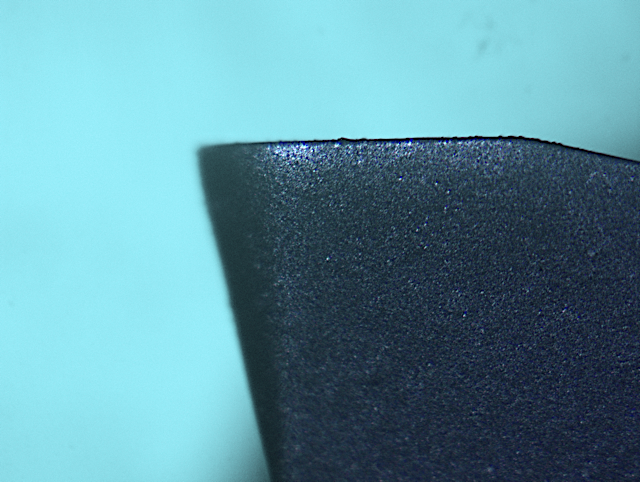
\includegraphics[width=\linewidth]{Tool_New_Insert.png}
    \caption{A tool-insert without wear}
    \label{fig:tool_new}
  \end{subfigure}\hfill
  \begin{subfigure}[t]{0.48\textwidth}
    \centering
    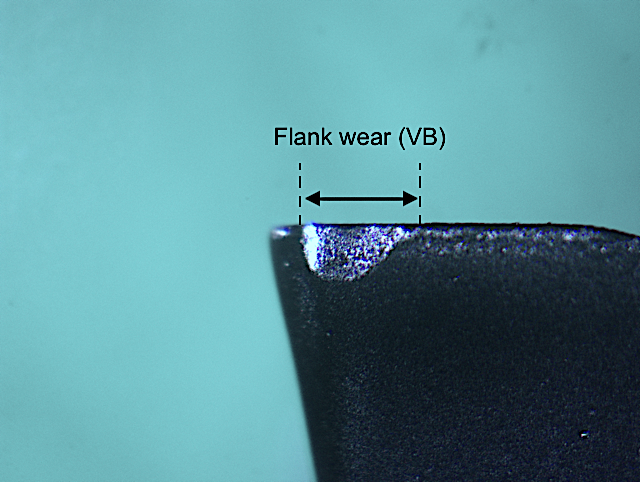
\includegraphics[width=\linewidth]{Tool_Worn Annotated.png}
    \caption{Tool-insert showing wear and how flank-wear (VB) is defined}
    \label{fig:tool_worn}
  \end{subfigure}
  \caption{Milling tool inserts - Digital images using tool-makers microscope}
  \label{fig:tool_images}
\end{figure}

\begin{figure}[t]
        \centering
        \includegraphics[width=0.48\textwidth]{dummy.pdf}\hfill
        \includegraphics[width=0.48\textwidth]{dummy.pdf}
        \caption{setup}
        \label{fig:machine-set-up}
\end{figure}


\begin{figure}[t]
  \centering
  \begin{subfigure}[t]{0.48\textwidth}
    \centering
    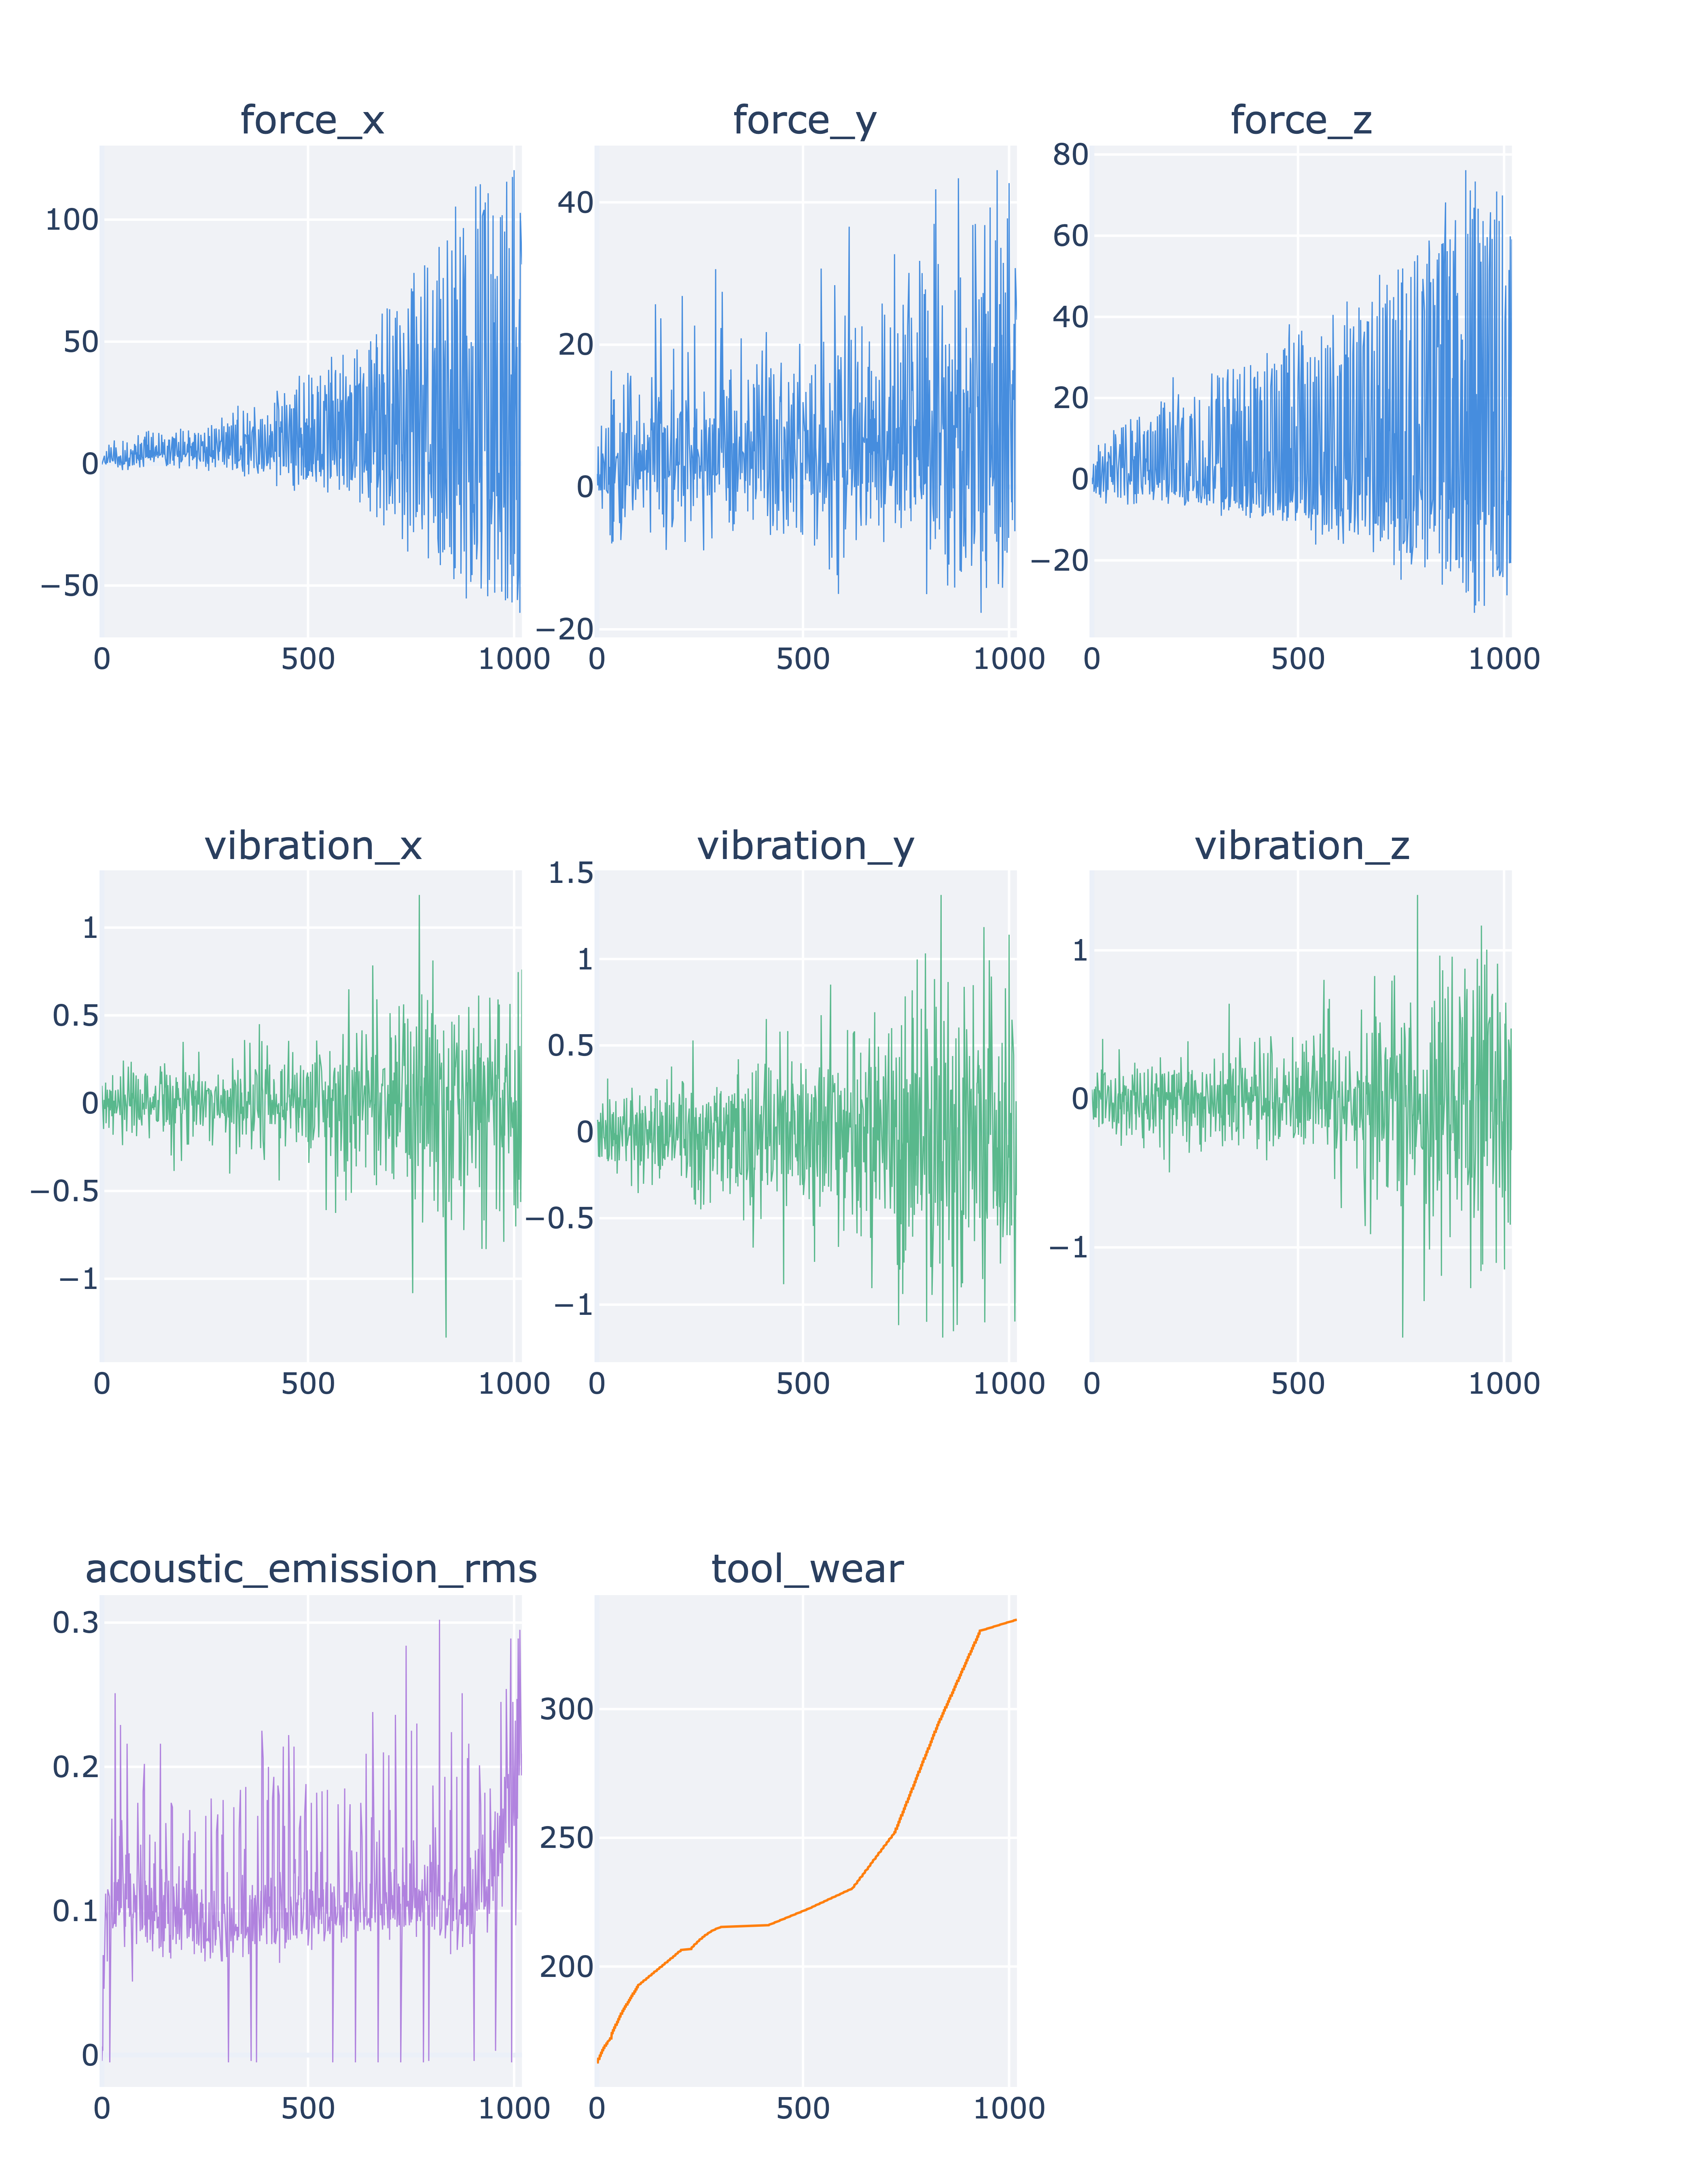
\includegraphics[width=\linewidth]{IEEE_06_SensorPlot.png}
    \caption{IEEE schema features.}
    \label{fig:schema_ieee}
  \end{subfigure}\hfill
  \begin{subfigure}[t]{0.48\textwidth}
    \centering
    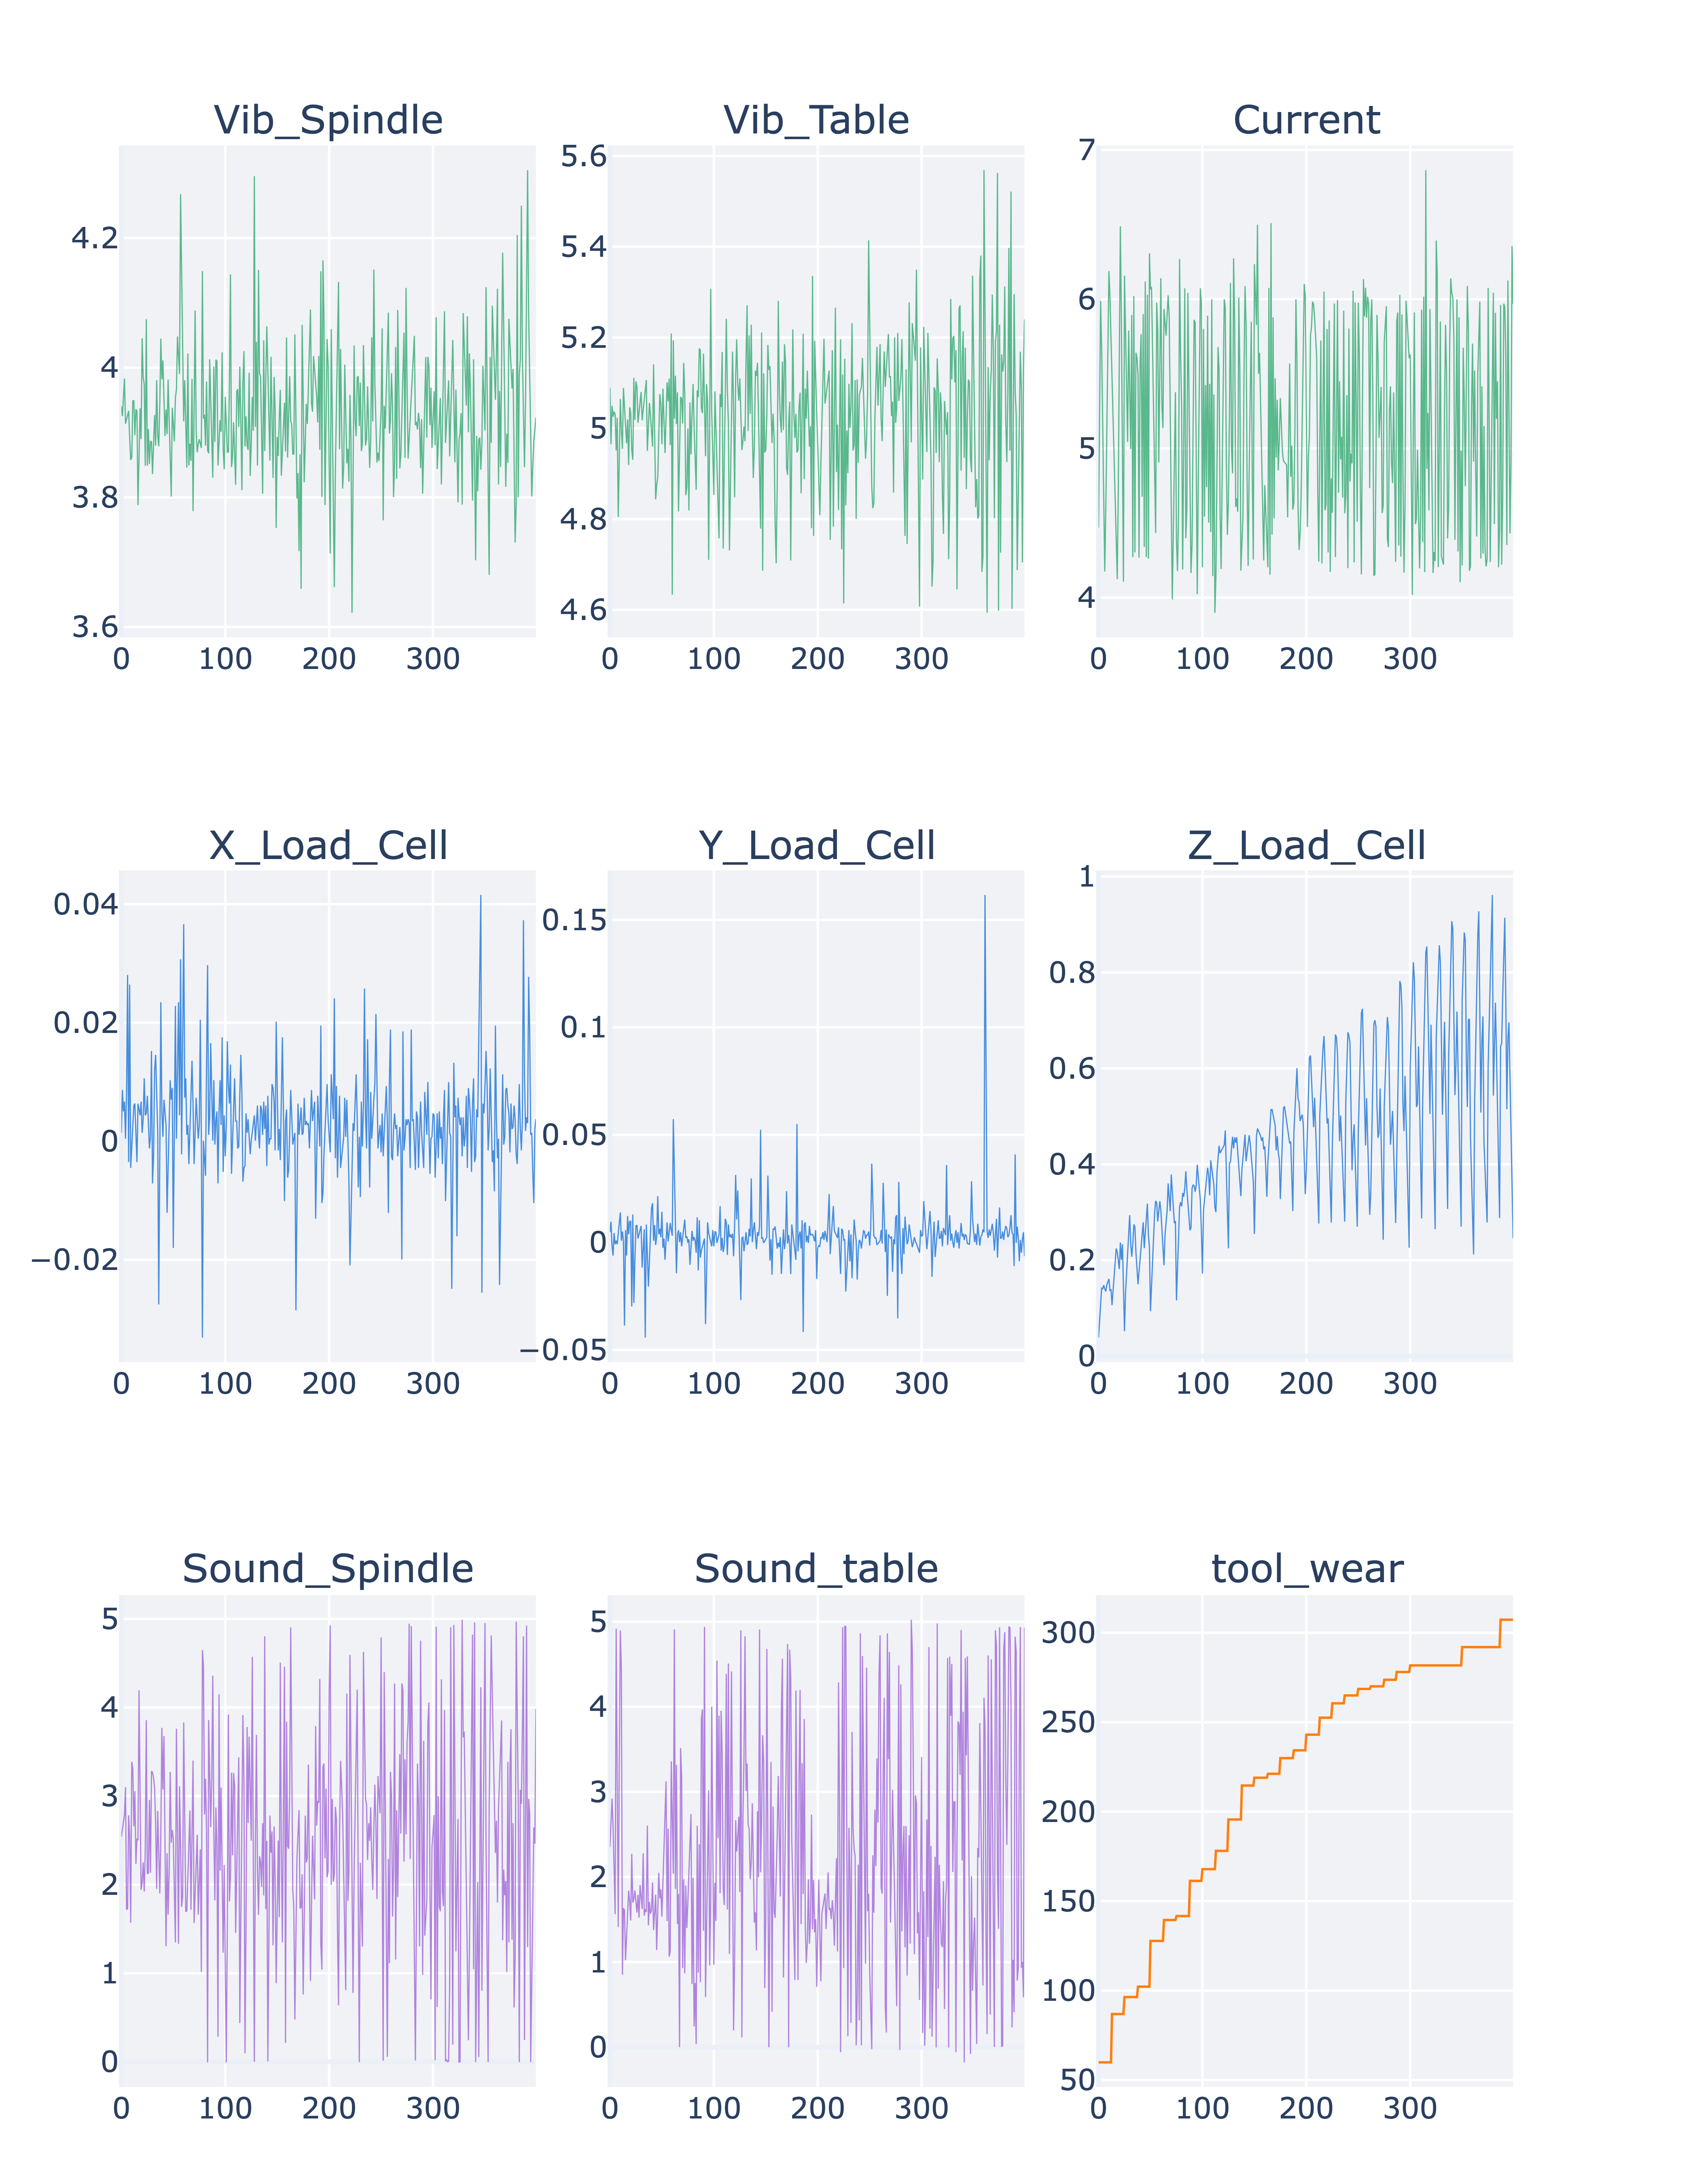
\includegraphics[width=\linewidth]{SIT_20_SensorPlot.png}
    \caption{SIT schema features.}
    \label{fig:schema_sit}
  \end{subfigure}

  \caption{IEEE and SIT schema feature plots: Representational plots depicting differences in sensor features, value ranges, and variations.}
  \label{fig:schema_feature_plots_ieee_sit}
\end{figure}

\begin{figure}[t]
        \centering
        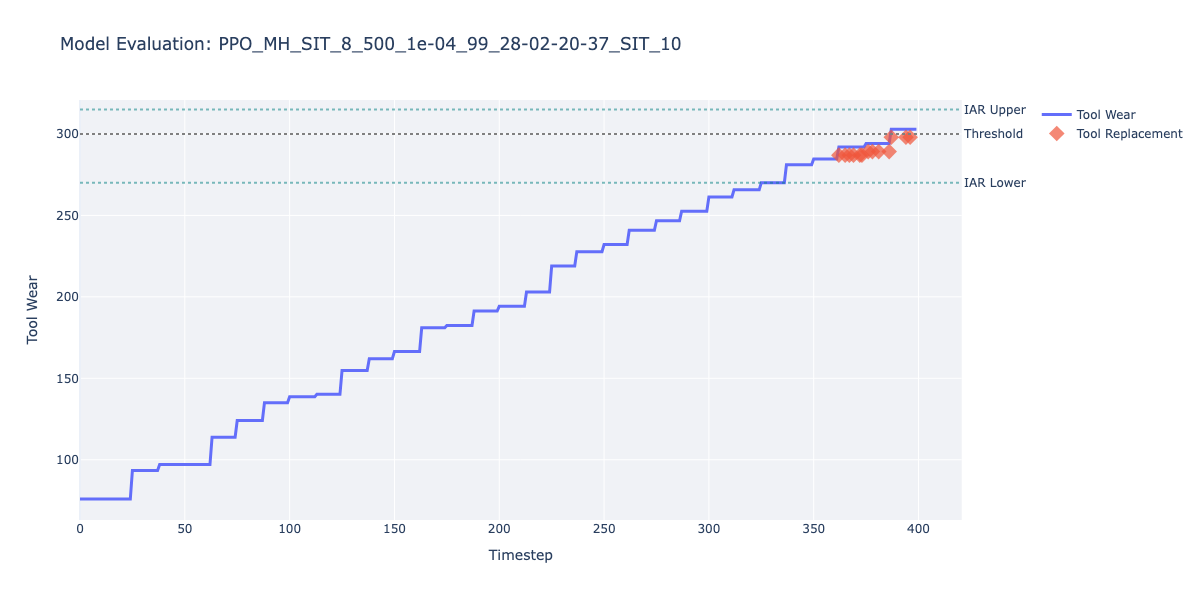
\includegraphics[width=0.48\textwidth]{PPO_MH_SIT_8_10.png}\hfill
        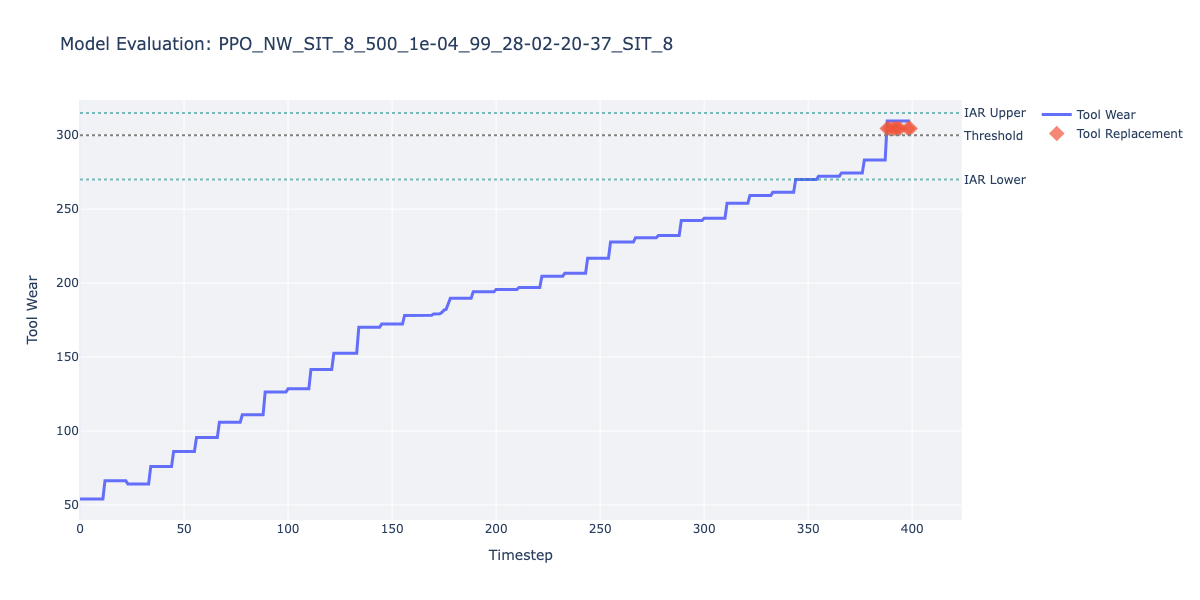
\includegraphics[width=0.48\textwidth]{PPO_NW_SIT_8_10.png}
        \caption{PPO trained PdM agents - evaluated on unseen data. \textbf{(a)} PPO with Multi-Head attention. \textbf{(b)} PPO with Nadaraya--Watson attention.}
        \label{fig:ppo_unseen_mh_nw}
\end{figure}

\section{Training strategy}
\huge\textcolor{red}{move later}
\normalsize
 - One - evaluate on rest\\
 - Single dataset - often combined of multiple experiments - but industrial practioners so did not combine.\\


\section{Background and related work}
\subsection{PdM, Industry~4.0, and edge constraints}
PdM is commonly positioned as an Industry~4.0 centerpiece because it links sensing, connectivity, analytics, and operational decision-making in cyber-physical production systems \cite{Compare2020, Zonta2020}. Prescriptive maintenance architectures further motivate this role by embedding decision-making (when to defer vs intervene) into cyber-physical workflows \cite{Ansari2019}. Edge deployment strengthens the PdM case by enabling low-latency, resilient operation near equipment, but it also introduces feasibility constraints: memory, compute, latency, and system-integration overhead can limit the practical adoption of complex ML/RL pipelines \cite{Njor2024, Pandey2023}. These constraints connect to sustainability and ``Green AI'' concerns: when many candidate agents are trained during AutoRL exploration, the incremental cost per training run becomes operationally and environmentally relevant \cite{Schwartz2020, Strubell2019}.

\subsection{RL for predictive maintenance}
RL has been surveyed extensively in PdM, with evidence that a wide range of formulations have been explored across maintenance scheduling, inspection, and resource-constrained decision problems \cite{Siraskar2023, Ogunfowora2023, Zhang2024}. A consistent theme across these surveys is that the ``right'' RL complexity level depends on (i) the structure of the decision problem (action-space size, horizon, coupling) and (ii) deployment realism (compute, memory, latency).

The literature also suggests a useful two-stream picture. Many PdM and condition-based maintenance studies learn effective policies using non-deep or otherwise lightweight RL, especially when state representations are structured and action spaces are modest \cite{Adsule2020, Yousefi2020, Rasay2024, Dadash2024}. Deep RL (e.g., DQN/PPO-style methods) becomes more prominent as environments become richer and harder: higher-dimensional sensing, long-horizon tradeoffs, multi-component scheduling, or coupled resource constraints \cite{Liu2020, Chen2023, Lee2022, Ong2022-02}.

\subsection{Positioning lightweight RL for edge PdM (qualified defense)}
The strongest literature-backed position is a \emph{qualified defense} of lightweight RL for edge PdM: the literature does not establish that REINFORCE is universally better than advanced deep RL, but it does support the claim that lightweight methods are often the more credible engineering choice when the PdM task is structured and edge constraints are first-order requirements \cite{Compare2020, Njor2024, Pandey2023}. In embedded RL more broadly, deep RL frequently requires additional machinery---transfer learning, pruning, compression, or distillation---to fit acutely constrained devices \cite{Jang2020, Szydlo2022, Xu2022}.

Sustainability motivations should also be framed carefully. Maintenance optimization can contribute to energy and emissions objectives in industrial systems, but the PdM literature rarely reports algorithm-level energy draw or carbon footprints for competing RL methods. Accordingly, ``Green AI'' claims in this paper are positioned as downstream implications of reduced computational demand and edge-feasible deployment, not as directly measured environmental outcomes \cite{Banyai2021, Banyai2022, JasiulewiczKaczmarek2024}.

The most direct quantitative anchor for this positioning is the recent empirical PdM study by Siraskar et al.~\cite{Siraskar2025}. Across 15 environment variants and 10 rounds of training and testing, REINFORCE achieved the highest reported tool-replacement precision at 0.687, exceeding the next-best method by 0.215 in absolute terms; the same study reports that REINFORCE also led the other algorithms on recall, F1, and $F_{\beta=0.5}$. The reported model sizes were small: 56.4~KB for DQN, 89.8~KB for A2C, 121.5~KB for REINFORCE, and 135.5~KB for PPO \cite{Siraskar2025}.

A second quantitative anchor comes from richer IIoT maintenance decision problems where heavier DRL can earn its place. Ong et al.~report that a PPO--LSTM based PdM framework outperformed comparable DRL methods by 53\% and human participants by 65\% in a maintenance resource-management simulator \cite{Ong2022-01}. In a follow-on study, the same line of work introduced transfer learning with demonstrations to reduce DRL training wall time by 58\% \cite{Ong2022-02}.

A third quantitative anchor comes from edge deployment studies that make the memory bottleneck concrete. Pandey et al.~show that in a PdM edge-deployment study, pruning could reduce model sizes dramatically while keeping the average accuracy drop within about 3 percentage points \cite{Pandey2023}. For example, with STFT features, AlexNet was reduced from 28,534,479 to 75,627 parameters (accuracy 98.37\% to 97.65\%), while LeNet fell from 76,695 to 1,967 parameters (accuracy 98.07\% to 97.13\%) \cite{Pandey2023}. With CWT features, AlexNet fell from 28,534,479 to 656,620 parameters \cite{Pandey2023}. The implication is not that deep models are unusable, but that their deployment often depends on pruning, quantization, distillation, or related compression steps before edge feasibility can be discussed \cite{Pandey2023, Jang2020, Xu2022}.

\begin{table}[t]
        \centering
        \small
        \setlength{\tabcolsep}{4pt}
        \begin{tabular}{p{0.24\textwidth} p{0.42\textwidth} p{0.30\textwidth}}
                \toprule
                Evidence strand & Quantitative anchor & Reviewer-safe reading \\
                \midrule
                Direct REINFORCE evidence in PdM & REINFORCE leads tool-replacement precision at 0.687 across 15 variants, and reported model sizes remain small (56.4~KB DQN, 89.8~KB A2C, 121.5~KB REINFORCE, 135.5~KB PPO) \cite{Siraskar2025} & A simple policy-gradient baseline can be competitive in PdM and is not disqualified on footprint grounds \\
                Richer IIoT maintenance decision problems & PPO--LSTM outperforms comparable DRL methods by 53\% and human participants by 65\% in a maintenance resource-management simulator \cite{Ong2022-01} & As the decision problem becomes richer and more coupled, heavier DRL can earn its place \\
                Cost of making DRL practical & Transfer learning with demonstrations cuts DRL training wall time by 58\% \cite{Ong2022-02} & Stronger DRL performance often comes with extra algorithmic machinery and training burden \\
                Edge deployment bottleneck & AlexNet with STFT features shrinks from 28,534,479 to 75,627 parameters with accuracy moving from 98.37\% to 97.65\% after pruning \cite{Pandey2023} & Memory headroom is a hard engineering constraint, not a vague concern \\
                \bottomrule
        \end{tabular}
        \caption{Quantitative anchors supporting a reviewer-safe positioning of lightweight RL for edge-aware PdM.}
        \label{tab:quantitative_anchors_lightweight_edge}
\end{table}

\subsection{AutoRL and practitioner-centered experimentation}
AutoRL refers to automating choices that otherwise require expert RL knowledge: algorithm selection, hyperparameter tuning, reward shaping, and robust evaluation. Prior work emphasizes that automation can improve performance and reproducibility, and can lower the barrier for non-expert adoption \cite{Faust2019, Mussi2022}. In industrial PdM settings, the motivation is pragmatic: practitioners often cannot afford extensive manual hyperparameter tuning cycles (time, compute, and expertise), so standardized sweeps and reporting become a credible adoption path, especially when compute cost is treated as a first-class concern \cite{Schwartz2020, Strubell2019}.

\subsection{Attention mechanisms for PdM}
Attention mechanisms reweight inputs to focus computation on the most relevant parts of an observation, and have become a standard architectural primitive in modern deep learning \cite{Vaswani2017}. In PdM, attention can be interpreted as a structured inductive bias that emphasizes salient sensor channels or degradation stages. The present study builds on prior PdM attention work that introduced a Nadaraya--Watson estimator based attention mechanism as a lightweight option aligned with edge constraints \cite{Siraskar2024}.

\subsection{Evidence synthesis: REINFORCE with attention for edge-aware PdM}
\label{sec:reinforce_attention_pdm}

Predictive maintenance in Industry~4.0 has moved beyond failure prediction toward prescriptive maintenance, where the central problem is to decide when to inspect, defer, repair, or replace under uncertainty \cite{Compare2020, Ansari2019, Siraskar2023, Zhang2024}. This shift makes reinforcement learning (RL) a natural methodological fit because maintenance is a sequential control problem rather than a purely predictive one. At the same time, many PdM deployments are expected to operate close to the asset or within IIoT pipelines, where memory, latency, and engineering overhead remain binding constraints \cite{Compare2020, Pandey2023, Njor2024}. The literature therefore supports a simple premise for the present study: in edge-aware PdM, the best method is not automatically the deepest one.

\subsubsection{RL for edge-oriented PdM}
A first layer of evidence shows that lightweight reinforcement learning is already credible in maintenance optimization. Non-deep or relatively simple RL formulations learn useful maintenance policies across multi-state machines, condition-based maintenance, and repairable multi-component systems \cite{Wang2014, Adsule2020, Yousefi2020}. Review work by Siraskar et al. consolidates this wider result and identifies REINFORCE as an underexplored but legitimate PdM direction \cite{Siraskar2023}. This shifts the burden of proof: a REINFORCE-based method does not need to justify RL itself, but rather why a lighter policy-gradient learner is sufficient for the target maintenance setting.

A second layer of evidence comes from edge-oriented PdM and IIoT deployment studies. Deep RL can perform strongly in richer resource-management and maintenance environments \cite{Ong2022-01, Ong2022-02}, but the same literature also reveals the cost of that power. Transfer learning is introduced to reduce DRL training wall time in IIoT-based manufacturing \cite{Ong2022-02}, while edge PdM deployment studies repeatedly report memory, pruning, quantization, and toolchain constraints before modern DNNs can run on microcontrollers or TinyML stacks \cite{Pandey2023, Njor2024}. The implication is not that deep RL is ineffective; rather, complexity must earn its place once deployment realism is treated as part of the evaluation criterion.

\subsubsection{The case for REINFORCE as a lightweight baseline}
Within this edge-aware framing, REINFORCE becomes a serious PdM candidate because it keeps the policy learner simple while preserving direct policy optimization. A direct anchor is Siraskar et al., who show that na\"{i}ve REINFORCE can be empirically competitive for predictive maintenance \cite{Siraskar2025}. That result sits on top of a broader maintenance literature in which simpler RL methods solve useful decision problems without a large algorithmic stack \cite{Wang2014, Adsule2020, Yousefi2020}. In literature-review terms, REINFORCE is best positioned not as a universal replacement for PPO, DQN, or other deep methods, but as a defensible lightweight baseline whose value rises when deployment feasibility matters.

\begin{table}[t]
        \centering
        \small
        \setlength{\tabcolsep}{4pt}
        \begin{tabular}{p{0.24\textwidth} p{0.42\textwidth} p{0.30\textwidth}}
                \toprule
                Evidence strand & Quantitative anchor & Reviewer-safe reading \\
                \midrule
                Direct REINFORCE anchor & 15 PdM environment variants, highest reported precision at 0.687, model size 121.5~KB \cite{Siraskar2025} & Lightweight policy learning is empirically credible \\
                Edge deployment pressure & Large PdM models require major pruning, for example 28,534,479 to 75,627 parameters with small accuracy loss in one STFT case \cite{Pandey2023} & Deep models may be deployable, but often only after substantial compression \\
                Embedded RL feasibility & Distillation and compression are introduced to obtain smaller edge policies with near-cloud reward and lower training burden \cite{Jang2020, Xu2022, Szydlo2022} & Constrained deployment is not free; it often requires extra method layers \\
                \bottomrule
        \end{tabular}
        \caption{Evidence chain 1 (quantitative anchors): lightweight RL for edge-aware PdM.}
        \label{tab:evidence_chain1_quant}
\end{table}

\subsubsection{The case for attention in PdM}
Attention mechanisms provide the representational argument: they can compress long and noisy sensor histories into a more decision-relevant state representation. In PdM, attention is well established for remaining useful life estimation, degradation tracking, and multi-sensor health modeling \cite{Chen2020, Chen2021, Chadha2022, DeLuca2023}. Importantly, this literature is not only about predictive accuracy. De Luca et al. show that an attention-based PdM model can offer a useful effectiveness--efficiency compromise for IoT execution \cite{DeLuca2023}. Xia et al. move attention closer to action support by coupling self-attention with rolling predictive maintenance decisions \cite{Xia2022}.

\begin{table}[t]
        \centering
        \small
        \setlength{\tabcolsep}{4pt}
        \begin{tabular}{p{0.24\textwidth} p{0.42\textwidth} p{0.30\textwidth}}
                \toprule
                Evidence strand & Quantitative anchor & Reviewer-safe reading \\
                \midrule
                Direct REINFORCE anchor & REINFORCE is competitive in PdM while remaining small in model size \cite{Siraskar2025} & A lightweight policy learner is already plausible \\
                Attention for efficient PdM representation & Attention-based PdM is framed as an effectiveness--efficiency compromise with smaller parameter count, smaller storage volume, and lower training time \cite{DeLuca2023} & Attention is relevant not only for accuracy, but also for efficient representation \\
                Attention linked to maintenance decisions & Self-attention is coupled with rolling predictive maintenance decisions over time \cite{Xia2022} & Attention can feed action support, not only RUL estimation \\
                Attention plus RL for maintenance actions & Published combinations use Transformer plus DQN, PPO, SAC, or related DRL stacks rather than REINFORCE \cite{Zhao2024, Zhang2023, Guo2026} & The combined literature exists, but it is concentrated on heavier architectures \\
                \bottomrule
        \end{tabular}
        \caption{Evidence chain 2 (quantitative anchors): from attention in PdM to REINFORCE with attention.}
        \label{tab:evidence_chain2_quant}
\end{table}

\begin{table}[t]
        \centering
        \small
        \begin{tabular}{p{0.21\textwidth} p{0.24\textwidth} p{0.24\textwidth} p{0.21\textwidth}}
                \hline
                Evidence layer & Core papers & What is already supported & What remains open \\
                \hline
                Edge-aware RL for PdM & \cite{Wang2014, Adsule2020, Yousefi2020, Ong2022-01, Ong2022-02} & RL is suitable for maintenance decision making, and deployment constraints matter for method choice & Whether a lightweight policy-gradient method can retain enough performance under edge-oriented conditions \\
                REINFORCE in PdM & \cite{Siraskar2025, Siraskar2023} & REINFORCE is a legitimate PdM method and now has direct empirical support & Whether representation quality limits a na\"{i}ve REINFORCE policy in richer sensor settings \\
                Attention in PdM & \cite{Chen2020, Chen2021, Chadha2022, DeLuca2023, Xia2022} & Attention improves temporal and sensor-wise representation in prognostics and related PdM tasks & Whether those representational gains transfer cleanly to maintenance-action learning \\
                Attention plus RL for maintenance actions & \cite{Zhao2024, Zhang2023, Guo2026} & Attention can strengthen maintenance decision learning under temporal complexity and partial observability & Existing evidence uses heavier DRL, DQN, PPO, SAC, or MARL rather than REINFORCE \\
                \hline
        \end{tabular}
        \caption{Evidence chain leading to the present study. The literature is strong on the two components and on adjacent combinations, but still thin at their exact intersection.}
        \label{tab:evidence_chain}
\end{table}

\subsubsection{The case for REINFORCE with attention}
The bridge from attention-based representation to maintenance-action learning has begun to appear, but it is still dominated by heavier deep RL designs. Transformer-driven prescriptive maintenance, counterfactual-attention multi-agent RL, and transformer-augmented DQN show that attention can improve maintenance decision learning under temporal complexity, partial observability, or joint scheduling demands \cite{Zhao2024, Zhang2023, Guo2026}. Yet these studies do not use REINFORCE. In parallel, Siraskar et al. provide direct evidence that REINFORCE can already be competitive in predictive maintenance without attention \cite{Siraskar2025}. Taken together, these two strands motivate a narrow and coherent research opening: attention can strengthen state representation, while REINFORCE preserves a lightweight policy learner.

\subsubsection{What the Scopus scoping queries add (and where they differ)}
To complement the narrative synthesis above, we ran two targeted Scopus scoping queries to check evidence density at two intersections relevant to this study.

First, for the intersection \emph{RL $\cap$ edge computing $\cap$ Industry~4.0 $\cap$ (predictive/preventive maintenance)}, the Scopus survey indicates five abstract-level hits in the screened set. These span (i) PdM frameworks that explicitly combine RL and edge/digital-twin themes \cite{Prabu2025, Pabitha2025}, (ii) PdM studies that use RL for health-state or maintenance decision learning \cite{Aglogallos2026}, and (iii) prescriptive maintenance comparisons deployed on edge computing nodes \cite{Tham2023}. One additional Scopus hit \cite{Khebbache2021} is an edge-RL application outside maintenance (virtualized face detection), which we treat as adjacent evidence about edge-RL feasibility rather than as PdM evidence.

Second, for the intersection \emph{RL $\cap$ attention mechanisms $\cap$ (predictive/preventive maintenance)}, the Scopus survey likewise indicates five hits in the screened set. These include attention-coupled deep RL for prescriptive maintenance \cite{Zhao2024}, multi-agent attention-based maintenance and scheduling \cite{Zhang2023, Yao2024}, hybrid transformer--DRL designs \cite{Nimma2024}, probabilistic prognostics paired with DRL for group maintenance \cite{Zeng2026}, and attention-enhanced representation learning paired with multi-agent RL for aeroengine maintenance strategies \cite{Wan2026}.

These Scopus scoping results refine (rather than replace) the evidence-chain conclusion in Table~\ref{tab:evidence_chain}. Scopus survey says that \emph{RL+attention} evidence for PdM/PM exists in multiple domains and is no longer rare; whereas the UnderMind synthesis says that the \emph{specific} intersection targeted here (attention plus a lightweight policy-gradient learner such as REINFORCE for maintenance-action PdM under edge-oriented constraints) remains thin, with published attention+RL evidence dominated by heavier DRL/MARL designs.

\begin{figure}[t]
        \centering
        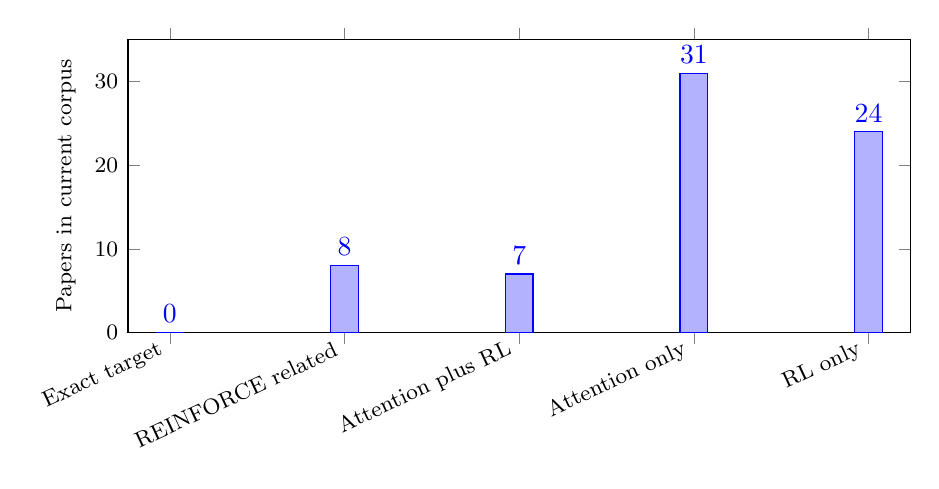
\begin{tikzpicture}
                \begin{axis}[
                                ybar,
                                bar width=10pt,
                                width=0.95\linewidth,
                                height=5.3cm,
                                ymin=0,
                                ymax=35,
                                ylabel={Papers in current corpus},
                                symbolic x coords={Exact target,REINFORCE related,Attention plus RL,Attention only,RL only},
                                xtick=data,
                                nodes near coords,
                                nodes near coords align={vertical},
                                enlarge x limits=0.06,
                                x tick label style={rotate=25,anchor=east,font=\footnotesize},
                                y tick label style={font=\footnotesize},
                                ylabel style={font=\footnotesize},
                                every axis plot/.append style={fill=black!65}
                        ]
                        \addplot coordinates {(Exact target,0) (REINFORCE related,8) (Attention plus RL,7) (Attention only,31) (RL only,24)};
                \end{axis}
        \end{tikzpicture}
        \caption{Evidence density in the current project corpus. The exact target combination is absent, while adjacent clusters are clearly populated. The counts reflect topic-level grouping in the present search corpus rather than a claim about the entire global literature.}
        \label{fig:evidence_sparsity}
\end{figure}

Figure~\ref{fig:evidence_sparsity} makes this structure visible for the present corpus: adjacent clusters are populated, but the exact REINFORCE+attention combination for maintenance-action PdM is absent. This absence should be read as a bounded gap claim (scoped to the present corpus and search strategy) rather than a universal first-ever claim. Even so, combining (i) direct REINFORCE evidence in PdM \cite{Siraskar2025}, (ii) mature attention evidence in PdM representation learning \cite{DeLuca2023, Chen2021, Xia2022}, and (iii) growing attention+RL evidence for maintenance-action learning in Scopus \cite{Zhao2024, Zhang2023, Wan2026} yields a conservative and journal-grade motivation: REINFORCE with attention is a natural next step that joins an edge-compatible policy learner with a representation mechanism already shown to be useful in predictive maintenance.

\section{Foundations: PdM as an MDP/POMDP and RL algorithms}
\label{sec:foundations}
\subsection{PdM as a decision process (MDP)}
\label{sec:mdp}
We model the milling-tool replacement task as an episodic Markov decision process (MDP)
$\mathcal{M}=\langle \mathcal{S},\mathcal{A},P,r,\gamma\rangle$ \cite{Sutton2018}.

\begin{itemize}
\item $\mathcal{S}$ is the (latent) state space capturing tool condition, operating parameters, and environment.
\item $\mathcal{A}=\{0,1\}$ is a binary action space with $a=0$ meaning \emph{replace} and $a=1$ meaning \emph{continue}.
\item $P(s'\mid s,a)$ is the transition kernel.
\item $r(s,a)$ is a shaped reward encoding asymmetric PdM costs (Section~\ref{sec:reward}).
\item $\gamma$ is the discount factor.
\end{itemize}

\subsection{Finite vs. infinite horizon and the discount factor \texorpdfstring{$\gamma$}{gamma}}
\label{sec:gamma}
\subsubsection{Infinite horizon}
In non-terminating environments ($\gamma\in[0,1)$), $\gamma$ must be strictly less than $1$ to ensure the discounted return converges.

\subsubsection{Finite horizon}
Predictive maintenance is naturally episodic: a rollout terminates when the tool is replaced or when a terminal failure/threshold event occurs. If the episode length is bounded by $T<\infty$, the cumulative return $\sum_{t=0}^{T}\gamma^t r_t$ is finite even when $\gamma=1$.

\subsection{Objective function, returns, and baselines}
\label{sec:objective}
The RL objective is to maximize expected discounted return under the policy $\pi_\theta$:
\begin{equation}
J(\theta)=\mathbb{E}_{\tau\sim\pi_\theta}\left[\sum_{t=0}^{T}\gamma^t r_t\right],
\end{equation}
where $\tau=(s_0,a_0,r_0,\ldots,s_T)$ is a trajectory.
Define the return from time $t$ as
\begin{equation}
G_t = \sum_{k=t}^{T} \gamma^{k-t} r_k.
\end{equation}
Policy-gradient methods often subtract a baseline $b(s_t)$ (e.g., a value function) from $G_t$ to reduce variance without changing the expected gradient.

\subsection{Partial observability in milling PdM (POMDP)}
\label{sec:pomdp}
In realistic PdM, the true health state (tool wear) is not directly observable at runtime. The environment therefore corresponds to a partially observable MDP (POMDP), where the agent receives an observation vector $o_t$ derived only from sensor channels and must infer the hidden wear variable $w_t$:
\begin{equation}
o_t = O(s_t) = \mathbf{x}_t, \qquad w_t \notin o_t.
\end{equation}
This design choice is implemented explicitly in the environment (Section~\ref{sec:env}), and motivates attention-based feature extraction (Section~\ref{sec:attention}) to improve inference from sensor streams.

\subsection{RL algorithms compared}
\label{sec:algos}
We compare four algorithms: DQN (value-based), A2C (actor--critic), PPO (policy optimization), and REINFORCE (Monte-Carlo policy gradient).

\subsubsection{REINFORCE (Monte-Carlo policy gradient)}
REINFORCE directly estimates the policy gradient using Monte-Carlo returns \cite{Williams1992}:
\begin{equation}
\nabla_\theta J(\theta) = \mathbb{E}\left[\sum_{t=0}^{T} \nabla_\theta \log \pi_\theta(a_t\mid s_t)\,\big(G_t-b(s_t)\big)\right].
\end{equation}

\subsubsection{A2C (advantage actor--critic)}
Actor--critic methods use a learned value baseline $V_\phi(s_t)$ to reduce variance. With advantage estimate $\hat{A}_t=G_t-V_\phi(s_t)$, the policy gradient takes the form
\begin{equation}
\nabla_\theta J(\theta) \approx \mathbb{E}\big[\nabla_\theta\log\pi_\theta(a_t\mid s_t)\,\hat{A}_t\big].
\end{equation}
The critic is trained by minimizing a regression loss such as
\begin{equation}
\mathcal{L}_V(\phi)=\mathbb{E}\big[(G_t - V_\phi(s_t))^2\big].
\end{equation}

\subsubsection{PPO (clipped policy optimization)}
PPO constrains policy updates using a clipped surrogate objective \cite{Schulman2017}. Define the probability ratio
\begin{equation}
 r_t(\theta)=\frac{\pi_\theta(a_t\mid s_t)}{\pi_{\theta_{\mathrm{old}}}(a_t\mid s_t)}.
\end{equation}
With advantage $\hat{A}_t$, the clipped objective is
\begin{equation}
\mathcal{L}^{\mathrm{CLIP}}(\theta)=\mathbb{E}\left[\min\Big(r_t(\theta)\hat{A}_t,\;\mathrm{clip}(r_t(\theta),1-\epsilon,1+\epsilon)\hat{A}_t\Big)\right].
\end{equation}
In typical implementations, the optimized objective also includes a value-function penalty and an entropy bonus:
\begin{equation}
\mathcal{J}(\theta,\phi)=\mathcal{L}^{\mathrm{CLIP}}(\theta) - c_1\,\mathcal{L}_V(\phi) + c_2\,H(\pi_\theta).
\end{equation}

\subsubsection{DQN (deep Q-learning)}
DQN learns an action-value function $Q_\theta(s,a)$ and minimizes a temporal-difference error with a target network \cite{Mnih2015}:
\begin{equation}
\mathcal{L}(\theta)=\mathbb{E}\left[\left(r_t + \gamma\max_{a'}Q_{\bar\theta}(s_{t+1},a') - Q_\theta(s_t,a_t)\right)^2\right].
\end{equation}
Experience replay and target-network updates stabilize learning, but partial observability can degrade performance without explicit memory.

\subsubsection{Why REINFORCE can be edge-suited}
When deployment constraints are first-order requirements, algorithmic simplicity can translate to smaller policies and lower training/inference overhead. In sweep-based experimentation (including AutoRL-style grids), simpler learners can also reduce total compute when many configurations must be compared. This does not guarantee superior reward, but it shifts the burden of proof: if a lightweight method is statistically competitive on PdM metrics, it may be preferable for edge-first deployments \cite{Schwartz2020, Njor2024}.

\section{Problem formulation: asymmetric costs and decision rationale}
\label{sec:problem}
PdM decisions are inherently asymmetric. A late replacement can cause defective parts, scrap, or catastrophic failure, while an early replacement wastes remaining tool life.

\begin{table}[t]
        \centering
        \caption{Conceptual cost-aware interpretation of PdM decisions (qualitative), aligned with the reward shaping in Section~\ref{sec:reward}.}
        \label{tab:cost_view}
        \begin{tabular}{p{0.18\linewidth} p{0.32\linewidth} p{0.42\linewidth}}
                \toprule
                \textbf{Case} & \textbf{Condition} & \textbf{PdM interpretation}\\
                \midrule
                Timely replace & $a_t=0$ near $w\approx\tau$ & Desired: high utilization and low violation risk.\\
                Early replace & $a_t=0$ when $w\ll\tau$ & Safe but wasteful: reduces risk while discarding useful life.\\
                Late action / violation & $a_t=1$ while $w>\tau$ & Worst case: elevated risk of quality loss or failure; strongly penalized.\\
                Continue safely & $a_t=1$ with $w<\tau$ & Encouraged: extracts remaining useful life when safe.\\
                \bottomrule
        \end{tabular}
\end{table}

\section{AutoRL as a practitioner convenience: standardized sweeps and reporting}
\label{sec:autorl}
The AutoRL pipeline is implemented as a CLI batch runner (\texttt{code/batch\_train.py}) that supports training, evaluation, and reporting across a grid of algorithms, hyperparameters, and attention mechanisms. The pipeline is designed to be practitioner-friendly in two ways:
\begin{itemize}
        \item \textbf{Automation:} algorithm and attention choices are enumerated automatically; evaluation is repeated for multiple rounds.
        \item \textbf{Reliability:} long-running sweeps use a lightweight SQLite checkpoint queue to recover from failures without manual intervention.
\end{itemize}
For this study, multi-round evaluation uses 20 rounds (\texttt{EVAL\_ROUNDS=20}) to support confidence intervals and statistical tests.

\section{Environment design: a Gymnasium-compatible milling PdM POMDP}
\label{sec:env}
\subsection{Design goals and schema abstraction}
The environment class \texttt{MT\_Env} (\texttt{code/rl\_pdm.py}) implements the Gymnasium interface \cite{Foundation2023}. A central design goal is schema generality: the same environment logic (episode structure, actions, and reward shaping) should work across different milling-machine sensor schemas.

In the implementation, schema abstraction is achieved by keeping the MDP ``skeleton'' fixed while allowing the observation \emph{feature set} to vary:
\begin{itemize}
        \item \textbf{Fixed across schemas:} the observation is a flat real-valued sensor vector $\mathbf{x}_t\in\mathbb{R}^d$, the action space is binary (replace vs. continue), and the reward/termination logic is driven by an internal wear threshold.
        \item \textbf{Schema-dependent:} the specific sensor columns used to form $\mathbf{x}_t$ (and therefore $d$) are selected based on column names.
\end{itemize}

\textbf{Schema detection.}
The environment detects the schema using available sensor columns (e.g., force and acoustic emission channels for IEEE; vibration, sound, and load-cell channels for SIT). If no known schema signature is found, the implementation falls back to using \emph{all} non-excluded columns as sensor features (excluding \texttt{Time}/\texttt{time}, \texttt{tool\_wear}, and \texttt{ACTION\_CODE}).

\textbf{Practical requirement for new datasets.}
To reuse \texttt{MT\_Env} on a new milling-machine dataset without code changes, the CSV must include a \texttt{tool\_wear} column (used internally for termination and reward) plus one or more numeric sensor columns (used as observations).

\subsection{Observation and action spaces}
Only sensor readings are included in the observation vector; \emph{tool wear} is excluded but retained internally for reward and termination. The action space is discrete with two actions: $a=0$ means \emph{replace} (terminates the episode) and $a=1$ means \emph{continue}.

\subsection{Reward shaping for asymmetric PdM risk}
\label{sec:reward}
The reward function encourages long tool use without threshold violation, while rewarding timely replacement close to the wear threshold. In the implementation, continuing yields a small positive survival reward $R_1$, violating the wear threshold yields a catastrophic penalty $R_2$, replacement has a small cost $R_3$, and replacement near the threshold earns a strong bonus $R_4$ (with stepped bonuses above 70\%, 80\%, and 90\% wear ratio).

This design reflects a practical PdM asymmetry: a late replacement causing quality loss or failure is substantially worse than an early replacement.

\section{Attention mechanisms as lightweight feature extractors}
\label{sec:attention}
Because wear is hidden from observation (Section~\ref{sec:pomdp}), the core challenge is representation learning from sensor vectors. We implement attention mechanisms as feature extractors $\phi_\theta(\mathbf{x}_t)$ that map a raw sensor vector into a compact embedding used by the RL policy.

\textbf{General attention concept.}
Given values $V=\{\mathbf{v}_1,\ldots,\mathbf{v}_n\}$ and a query $\mathbf{q}$, attention forms a convex combination
\begin{equation}
\mathrm{Attention}(\mathbf{q},V)=\sum_{i=1}^{n}\alpha_i\,\mathbf{v}_i,\qquad \sum_i\alpha_i=1,\;\alpha_i\ge 0,
\end{equation}
with weights computed by a softmax over a compatibility score $s(\mathbf{q},\mathbf{v}_i)$:
\begin{equation}
\alpha_i = \frac{\exp(s(\mathbf{q},\mathbf{v}_i))}{\sum_{j=1}^n\exp(s(\mathbf{q},\mathbf{v}_j))}.
\end{equation}

\textbf{Note on terminology.}
We use ``attention'' as a unifying design label for feature extractors that implement (i) learned reweighting/gating and (ii) structured fusion of sensor features and (optionally) time context.
\subsection{Nadaraya--Watson attention (NW)}
NW attention can be interpreted as kernel-regression-based soft retrieval from learnable prototypes. This mechanism is computationally light and aligns with prior PdM attention work motivated by edge constraints \cite{Siraskar2024}.

A standard Gaussian-kernel form is
\begin{equation}
\alpha_i = \frac{\exp\left(-\tfrac{\lVert \mathbf{k}_i-\mathbf{q}\rVert^2}{2\sigma^2}\right)}{\sum_j \exp\left(-\tfrac{\lVert \mathbf{k}_j-\mathbf{q}\rVert^2}{2\sigma^2}\right)},
\qquad \mathbf{z}=\sum_i\alpha_i\,\mathbf{v}_i.
\end{equation}

\begin{algorithm}[t]
\caption{NW attention feature extractor (forward pass)}
\label{alg:nw_forward}
\begin{algorithmic}[1]
\Require observation vector $\mathbf{x}$; learnable prototype keys $\{\mathbf{k}_i\}$ and values $\{\mathbf{v}_i\}$; query network $f_\theta$; parameter $\log\beta$
\Ensure context feature $\mathbf{z}$
\State $\mathbf{q} \gets f_\theta(\mathbf{x})$ \Comment{query}
\For{$i \gets 1$ to $N$}
        \State $d_i \gets \lVert \mathbf{q}-\mathbf{k}_i\rVert^2$
\EndFor
\State $\beta \gets \exp(\log\beta)$ \Comment{enforce $\beta>0$}
\State $\alpha \gets \mathrm{softmax}(-\beta\,\mathbf{d})$ \Comment{normalize over prototypes}
\State $\mathbf{z} \gets \sum_{i=1}^{N} \alpha_i\,\mathbf{v}_i$
\State \Return $\mathbf{z}$
\end{algorithmic}
\end{algorithm}

\subsection{Temporal attention (TP)}
Temporal attention injects an explicit stage-of-life signal using sinusoidal positional encodings and a learnable temporal embedding \cite{Vaswani2017}.

\begin{algorithm}[t]
\caption{Temporal attention feature extractor (forward pass)}
\label{alg:tp_forward}
\begin{algorithmic}[1]
\Require observation vector $\mathbf{x}$; spatial attention network $g_\theta$; positional encodings $\mathrm{PE}[\cdot]$; temporal embedding $\mathbf{e}$; timestep counter $t$; fusion network $h_\theta$
\Ensure feature embedding $\mathbf{z}$
\State $\mathbf{w} \gets g_\theta(\mathbf{x})$ \Comment{per-channel spatial weights}
\State $\tilde{\mathbf{x}} \gets \mathbf{x} \odot \mathbf{w}$
\State $\mathbf{p} \gets \mathrm{PE}[t \bmod T_{\max}] + \mathbf{e}$
\State $\mathbf{z} \gets h_\theta(\mathrm{concat}(\tilde{\mathbf{x}},\mathbf{p}))$
\State $t \gets t+1$
\State \Return $\mathbf{z}$
\end{algorithmic}
\end{algorithm}

\subsection{Multi-head attention (MH)}
Multi-head attention uses multiple attention heads to represent different subspaces of sensor relationships \cite{Vaswani2017}.

In standard form,
\begin{align}
\mathrm{head}_h &= \mathrm{Attention}(QW_h^Q,\,KW_h^K,\,VW_h^V),\\
\mathrm{MultiHead}(Q,K,V) &= \mathrm{Concat}(\mathrm{head}_1,\ldots,\mathrm{head}_H)\,W^O.
\end{align}

\begin{algorithm}[t]
\caption{Multi-head attention feature extractor (forward pass; head-gating over $H$ heads)}
\label{alg:mh_forward}
\begin{algorithmic}[1]
\Require observation vector $\mathbf{x}$; projections $W^Q,W^K,W^V$; output projection $W^O$; number of heads $H$; per-head dimension $d$; scale factor $c$
\Ensure feature embedding $\mathbf{z}$
\State $Q \gets (\mathbf{x}W^Q) \rightarrow \text{reshape}(H, d)$
\State $K \gets (\mathbf{x}W^K) \rightarrow \text{reshape}(H, d)$
\State $V \gets (\mathbf{x}W^V) \rightarrow \text{reshape}(H, d)$
\For{$h \gets 1$ to $H$}
        \State $s_h \gets c\,\langle Q_h, K_h\rangle$
\EndFor
\State $\alpha \gets \mathrm{softmax}(\mathbf{s})$ \Comment{normalize over heads}
\For{$h \gets 1$ to $H$}
        \State $\tilde{V}_h \gets \alpha_h\,V_h$
\EndFor
\State $\mathbf{z} \gets (\mathrm{concat}(\tilde{V}_1,\ldots,\tilde{V}_H))W^O$
\State \Return $\mathbf{z}$
\end{algorithmic}
\end{algorithm}

\subsection{Self-attention (SA)}
Self-attention projects the observation into a feature space and uses a compact Transformer-style block with residual connections and layer normalization.

In standard token-wise form,
\begin{equation}
\mathrm{SelfAttn}(X)=\mathrm{softmax}\left(\frac{XW_Q(XW_K)^\top}{\sqrt{d}}\right)XW_V.
\end{equation}

In this codebase, the softmax normalization is across the \emph{batch} dimension; this can act as a stabilization/gating mechanism, though it differs from token-wise self-attention.

\begin{algorithm}[t]
\caption{Self-attention feature extractor (forward pass; batch-normalized gating)}
\label{alg:sa_forward}
\begin{algorithmic}[1]
\Require mini-batch $\{\mathbf{x}_i\}_{i=1}^{B}$; projections $W^{\mathrm{in}},W^Q,W^K,W^V$; scale factor $c$; FFN; layer norms $\mathrm{LN}_1,\mathrm{LN}_2$
\Ensure output features $\{\mathbf{y}_i\}_{i=1}^{B}$
\For{$i \gets 1$ to $B$}
        \State $\mathbf{h}_i \gets \mathbf{x}_i W^{\mathrm{in}}$
        \State $\mathbf{q}_i \gets \mathbf{h}_i W^Q$; $\mathbf{k}_i \gets \mathbf{h}_i W^K$; $\mathbf{v}_i \gets \mathbf{h}_i W^V$
        \State $s_i \gets c\,\langle \mathbf{q}_i,\mathbf{k}_i\rangle$ \Comment{scalar compatibility score}
\EndFor
\State $\alpha \gets \mathrm{softmax}(\mathbf{s})$ \Comment{normalize across batch index $i$}
\For{$i \gets 1$ to $B$}
        \State $\tilde{\mathbf{v}}_i \gets \alpha_i\,\mathbf{v}_i$
        \State $\mathbf{u}_i \gets \mathrm{LN}_1(\mathbf{h}_i + \tilde{\mathbf{v}}_i)$
        \State $\mathbf{y}_i \gets \mathrm{LN}_2(\mathbf{u}_i + \mathrm{FFN}(\mathbf{u}_i))$
\EndFor
\State \Return $\{\mathbf{y}_i\}_{i=1}^{B}$
\end{algorithmic}
\end{algorithm}

\section{Experimental design}
\label{sec:experiment}

\subsection{\textcolor{red}{Machine description}}

Parameter/ Equipment used: Specification/Values\\
-------------
Machine : Vertical Milling Centre (VMC) Jyoti NVU PX10 \\
Vibration Sensor : vbr1/d0-3v (Micro detectors)\\
Sensors used: Vibration, Dynamometer, Current\\
Tool wear measurement: Radical Tool makers Microscope\\
Data Acquisition: National Instruments (NI) data acquisition system\\
Cutting Tool: Inserted End-mill Cutter (material-Tungsten Carbide)\\
Spindle Speed (rpm): 800, 900, 1000, 1100, 1200 \\
Feed Rate (mm/min): 20, 25, 30, 35, 40\\
Maximum allowable flank wear (mm): 0.32 mm\\

%% $$$ 

\begin{figure}[h]
        \centering
        \includegraphics[width=0.305\linewidth]{Expt_Setup_MillingMachine.png}
        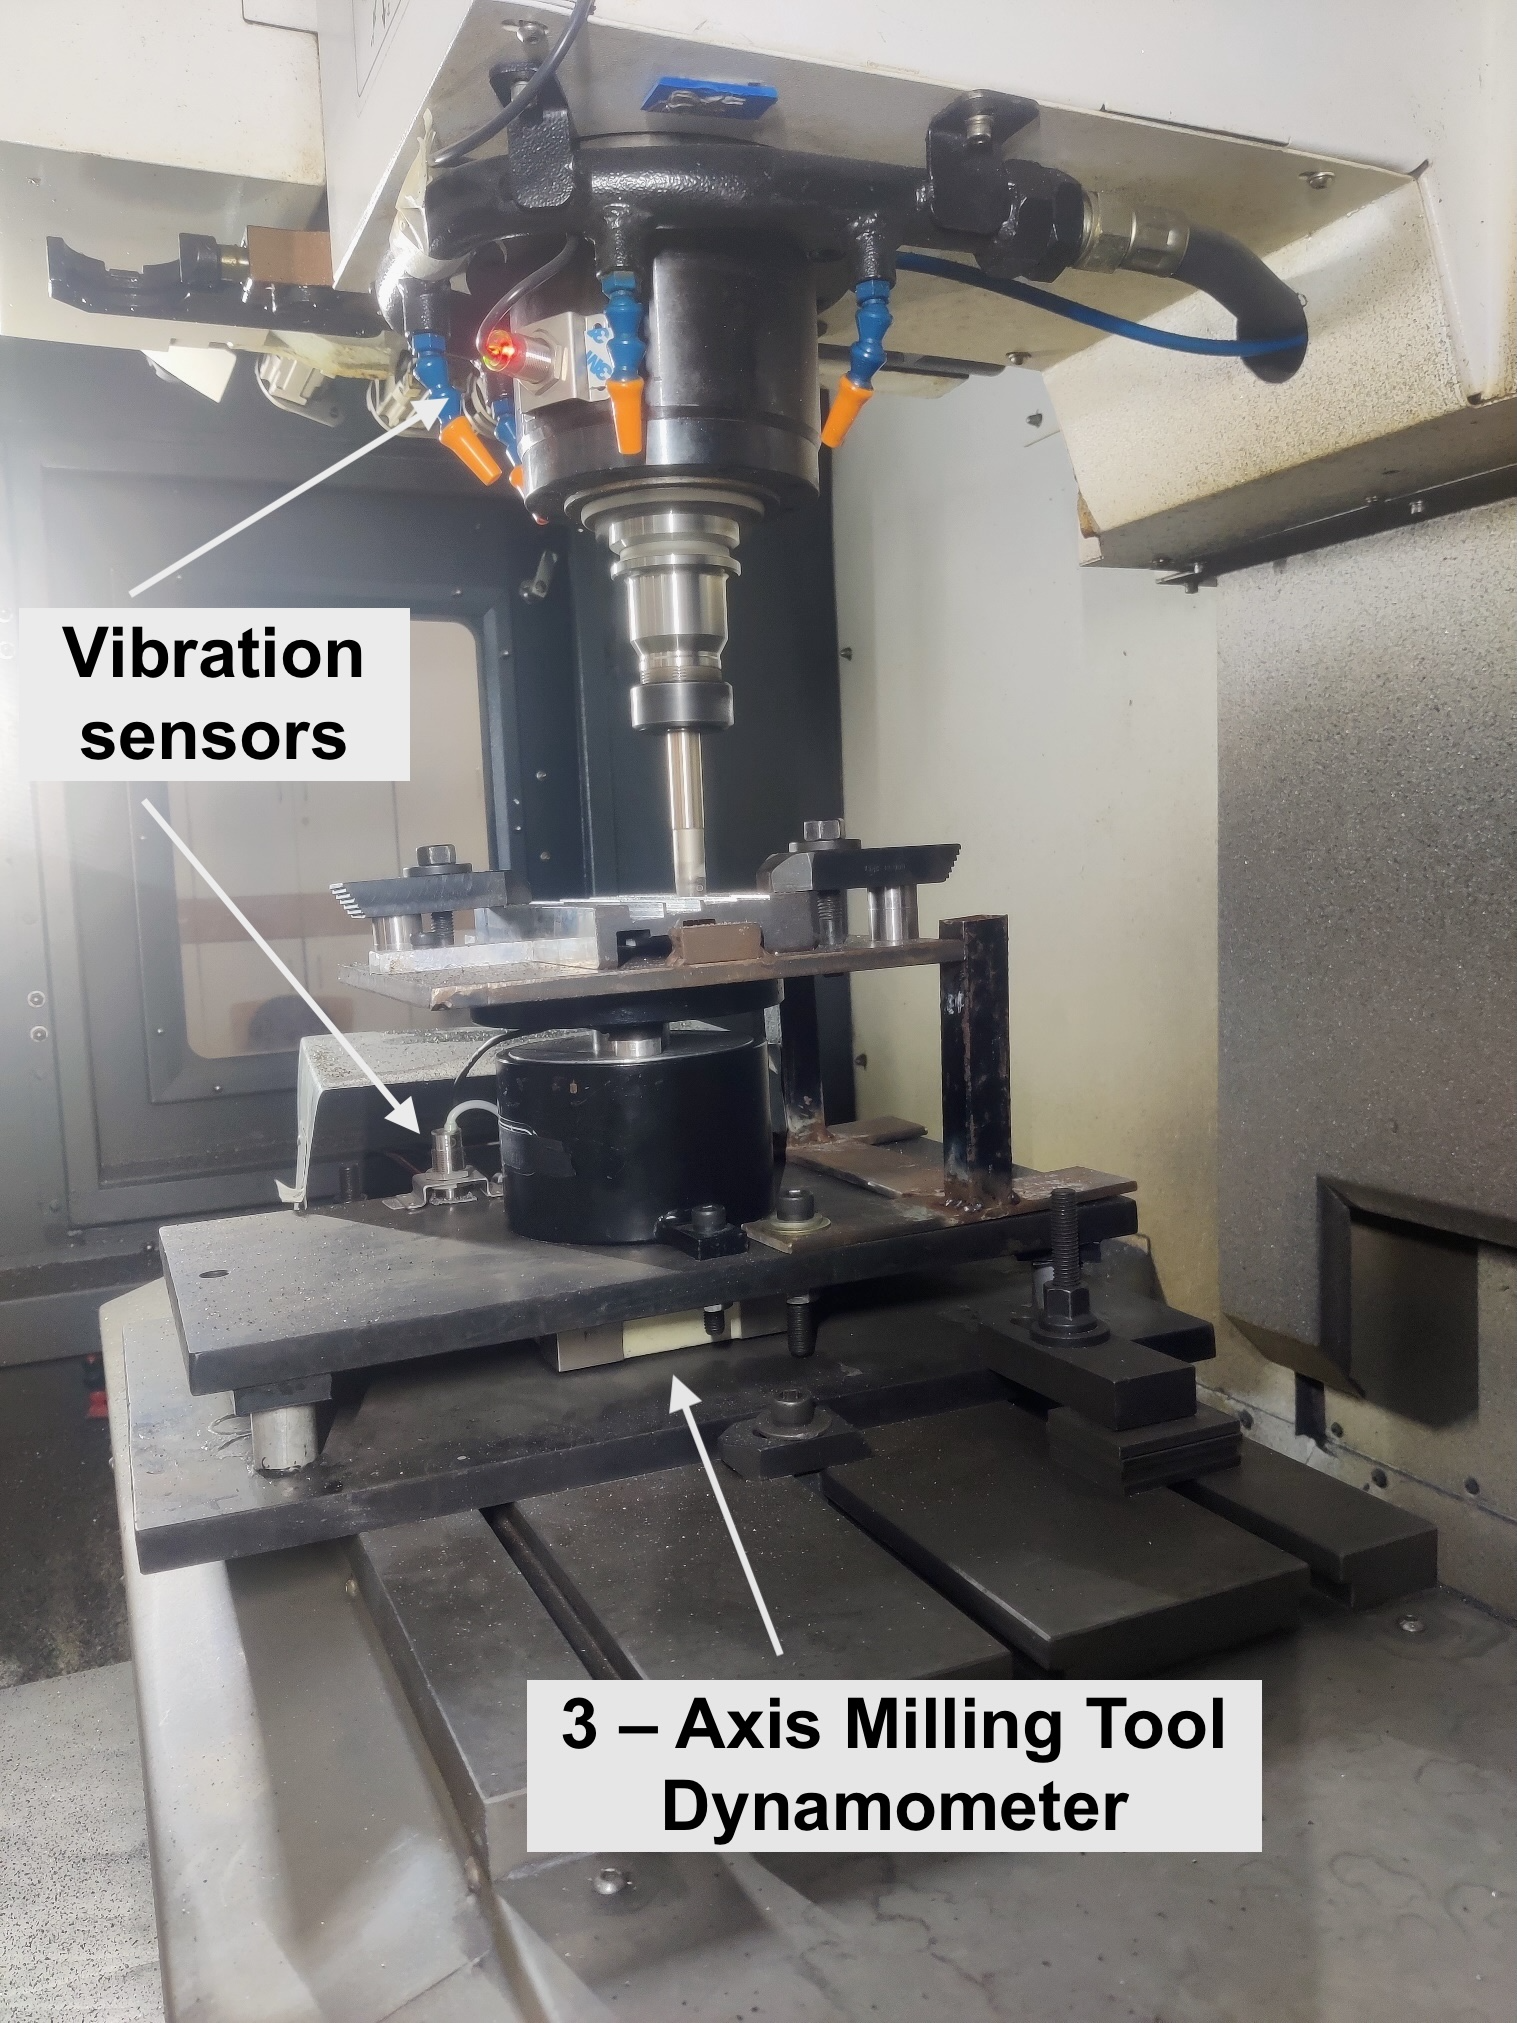
\includegraphics[width=0.45\linewidth]{Expt_Setup_Vibration_and_Dynamometer.png}
        \caption{Experimental setups}
        \label{fig:expt-setup-1}
\end{figure}

\begin{figure}[h]
        \centering
        \includegraphics[width=0.45\textwidth]{Expt_Setup_DACS.png}
        \includegraphics[width=0.445\textwidth]{Expt_Setup_Microscope.png}
        \caption{Experimental setups - measurement}
        \label{fig:expt-setup-2}
\end{figure}

\begin{table}[h!]
    \centering
    \caption{Progressive tool wear. Images taken using tool-makers microscope}
    \label{tab:wearimages}
    \begin{tabular}{|r|r|c|}
        \hline
        Runs & Wear $VB_{max}\mu$m & Tool condition\\
        \hline
         0 &   0.00 & 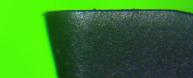
\includegraphics[width=0.3\linewidth]{tw-1.jpg} \\ \hline
         5 & 119.71 & 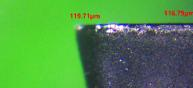
\includegraphics[width=0.3\linewidth]{tw-2.jpg} \\ \hline
        10 & 170.07 & 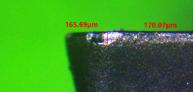
\includegraphics[width=0.3\linewidth]{tw-3.jpg} \\ \hline
        15 & 212.21 & 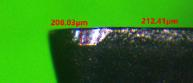
\includegraphics[width=0.3\linewidth]{tw-4.jpg} \\ \hline
        20 & 236.50 & 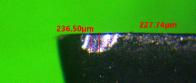
\includegraphics[width=0.3\linewidth]{tw-5.jpg} \\ \hline
        25 & 254.74 & 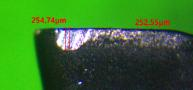
\includegraphics[width=0.3\linewidth]{tw-6.jpg} \\ \hline
        30 & 280.29 & 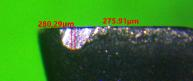
\includegraphics[width=0.3\linewidth]{tw-7.jpg} \\ \hline
        35 & 303.65 & 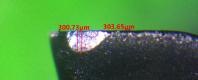
\includegraphics[width=0.3\linewidth]{tw-8.jpg} \\ \hline
    \end{tabular}
\end{table}


NUAA IdeahouseDatasetc - Eight  (Four-cutting forces, two vibrations, two current/power)\\
In-house Experimental Dataset : Six (Three-cutting forces, two vibrations, One current)\\

\subsection{Datasets and generalization protocol}
The study uses two sensor schemas: (i) SIT (production-oriented schema with eight sensor channels), and (ii) IEEE (benchmark schema with force, vibration, and acoustic emission channels). Generalization is evaluated via a one-vs-all protocol: agents are trained on training file(s) within a schema and evaluated on remaining unseen files within the same schema.

\subsection{Evaluation metrics}
\label{sec:metrics}
We report three metrics used by the AutoRL evaluation: (i) evaluation score, (ii) tool usage (\%), and (iii) a $\lambda$ timing metric.

\subsubsection{Exact evaluation score definition (as implemented)}
The paper-level ``evaluation score'' corresponds to \texttt{calculate\_eval\_score()} in \texttt{code/batch\_train.py}. Let $u\in[0,1]$ be tool usage fraction at first replacement, $v\in\mathbb{N}_0$ be the number of post-threshold timesteps without replacement (threshold violations), and $\lambda=t_{\lambda}-t_{\mathrm{FR}}$ be the signed timing error. The implemented score is
\begin{align}
S_{\text{tool}} &= \mathrm{clip}(u,0,1),\\
S_{\lambda} &= \max\left(0,\,1-\frac{|\lambda|}{c_{\lambda}}\right),\\
S_{\text{viol}} &= \frac{1}{1+v},\\
\mathrm{EvalScore} &= 0.50\,S_{\text{tool}} + 0.30\,S_{\lambda} + 0.20\,S_{\text{viol}}.
\end{align}
Here $c_{\lambda}$ is the normalization constant used by \texttt{calculate\_eval\_score()}, implemented as $c_{\lambda}=\texttt{WEAR\_THRESHOLD}\,(1-\texttt{IAR\_RANGE})$.

\begin{algorithm}[t]
\caption{Evaluation score computation (per evaluation run)}
\label{alg:eval_score}
\begin{algorithmic}[1]
\Require tool usage fraction $u$; timing error $\lambda$; violation count $v$; constants $c_{\lambda}=\texttt{WEAR\_THRESHOLD}\,(1-\texttt{IAR\_RANGE})$
\Ensure scalar score $S\in[0,1]$
\State $S_{\mathrm{tool}} \gets \mathrm{clip}(u, 0, 1)$
\State $S_{\lambda} \gets \max\left(0, 1 - \frac{|\lambda|}{c_{\lambda}}\right)$
\State $S_{\mathrm{viol}} \gets \max\left(0, \frac{1}{1+v}\right)$
\State $S \gets 0.50\,S_{\mathrm{tool}} + 0.30\,S_{\lambda} + 0.20\,S_{\mathrm{viol}}$
\State \Return $S$
\end{algorithmic}
\end{algorithm}

\subsubsection{Lambda metric and offline prognostic evaluation}
We implement a timing metric inspired by offline prognostic evaluation concepts \cite{Saxena2010Metrics}. Define $t_{\lambda}$ as the first timestep where wear exceeds an ``in-advance replacement'' (IAR) lower bound. Let $t_{\mathrm{FR}}$ be the first replacement timestep. Then
\begin{equation}
        \lambda = t_{\lambda} - t_{\mathrm{FR}}.
\end{equation}

\subsection{Multi-round evaluation, confidence intervals, and hypothesis tests}
For SIT, each trained model is evaluated for 20 rounds on unseen data to quantify variance from stochastic action sampling. Hypothesis testing uses one-tailed Welch $t$-tests (provided as CSV artefacts) at $\alpha=0.05$.

\textbf{Aggregation and 95\% confidence intervals.}
Let $S_1,\ldots,S_n$ denote the evaluation scores obtained across rounds and test files in a given panel. We report the sample mean and standard deviation
\begin{align}
\mu &= \frac{1}{n}\sum_{i=1}^{n} S_i,\\
\sigma &= \sqrt{\frac{1}{n-1}\sum_{i=1}^{n}(S_i-\mu)^2},
\end{align}
and the standard error of the mean $\mathrm{SEM}=\sigma/\sqrt{n}$. A normal-approximation 95\% CI is then $[\mu-1.96\,\mathrm{SEM},\;\mu+1.96\,\mathrm{SEM}]$.

\textbf{Statistical caveats.}
The $t$-tests are used as a practical, automated comparison tool for the AutoRL grid and should be interpreted with standard cautions: (i) multiple comparisons are performed across algorithms/attention panels and no correction is applied, and (ii) repeated evaluation rounds on the same test file can introduce dependence (pseudoreplication). Accordingly, the statistical panels are best treated as evidence of consistent trends rather than as definitive confirmatory inference.

\section{Results}
\label{sec:results}
This section reports consolidated evidence from the SIT and IEEE experiments using AutoRL dashboards, generalization heatmaps, and hypothesis-test artefacts.

\textbf{Experimental design for robustness.}
For SIT, we evaluate a consolidated set of results using 14 trained models and 14 evaluation files, with 20 stochastic evaluation rounds per model--file pair. For IEEE, we report results over 5 trained models and 5 evaluation files.

\subsection{Visual summaries: analysis dashboards and generalization heatmaps}
Figure~\ref{fig:analysis_sit} and Figure~\ref{fig:analysis_ieee} provide consolidated dashboards for each schema. Figure~\ref{fig:heatmap_sit} and Figure~\ref{fig:heatmap_ieee} complement these dashboards with one-vs-all generalization heatmaps.

\begin{figure}[t]
        \centering
        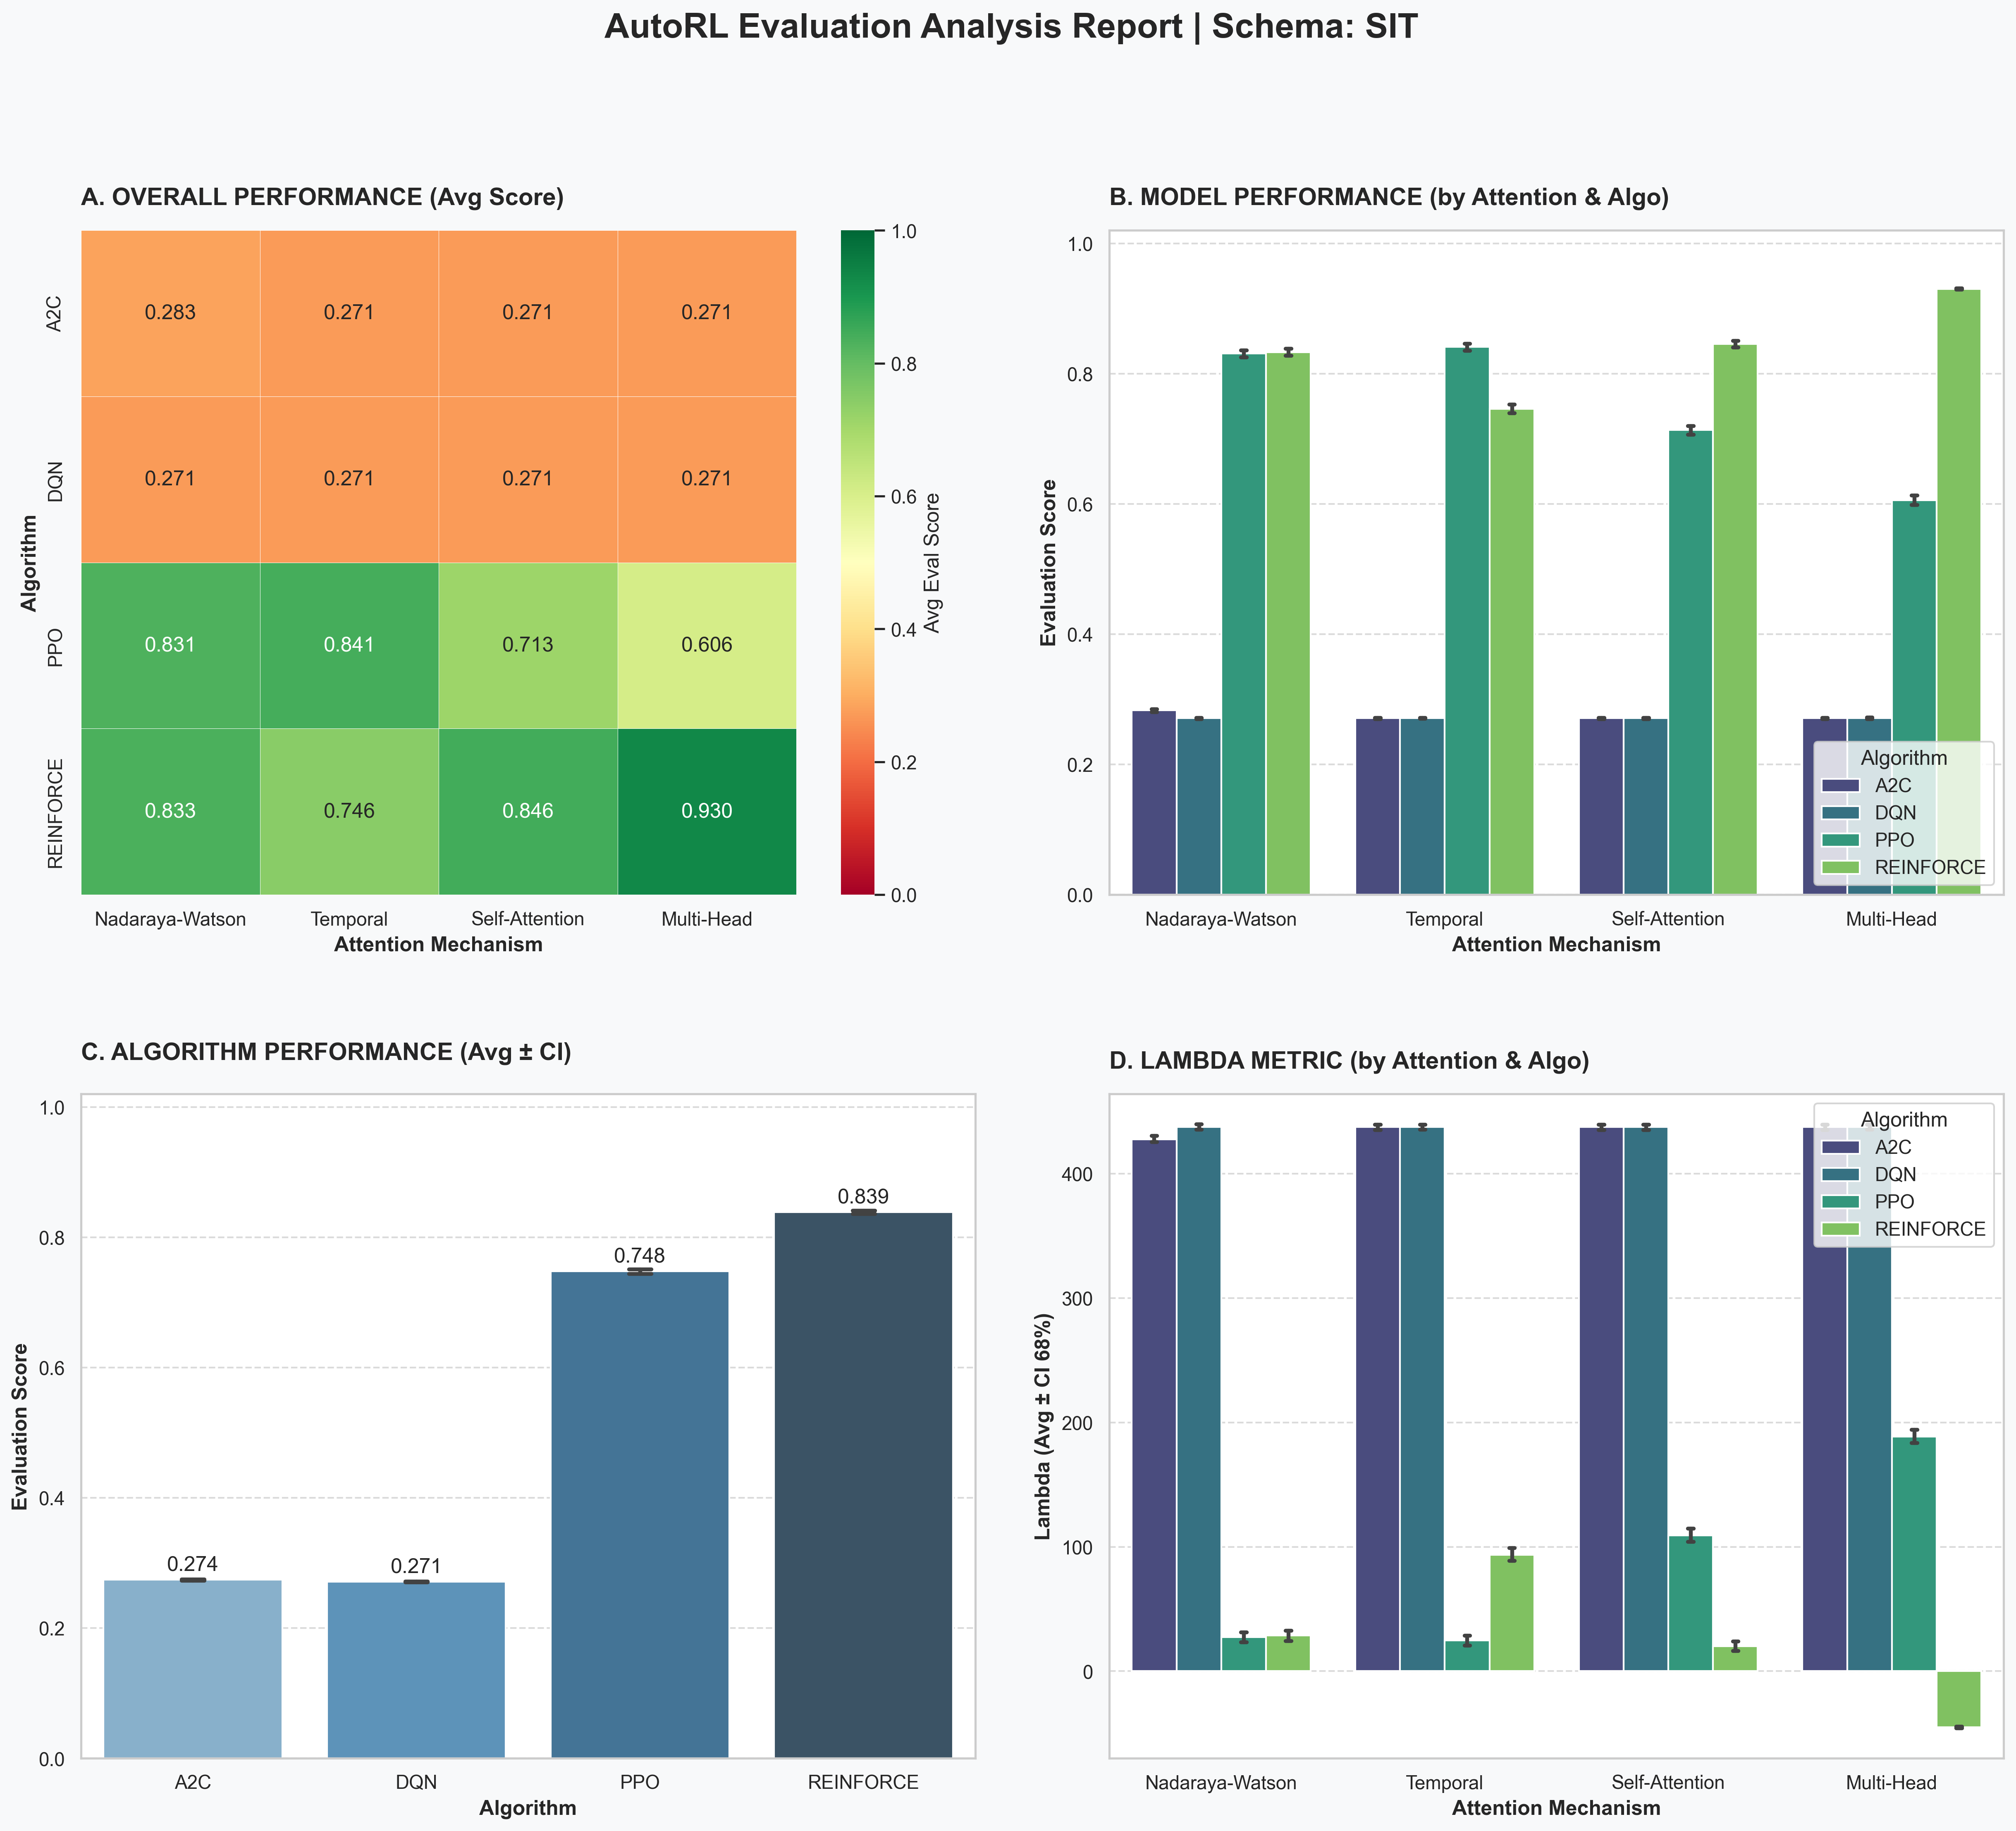
\includegraphics[width=0.95\textwidth]{_Analysis_Report_SIT.png}
        \caption{Consolidated evaluation dashboard for SIT (mean and uncertainty/error bars) used as primary visual evidence for performance patterns across algorithms and attention mechanisms.}
        \label{fig:analysis_sit}
\end{figure}

\begin{figure}[t]
        \centering
        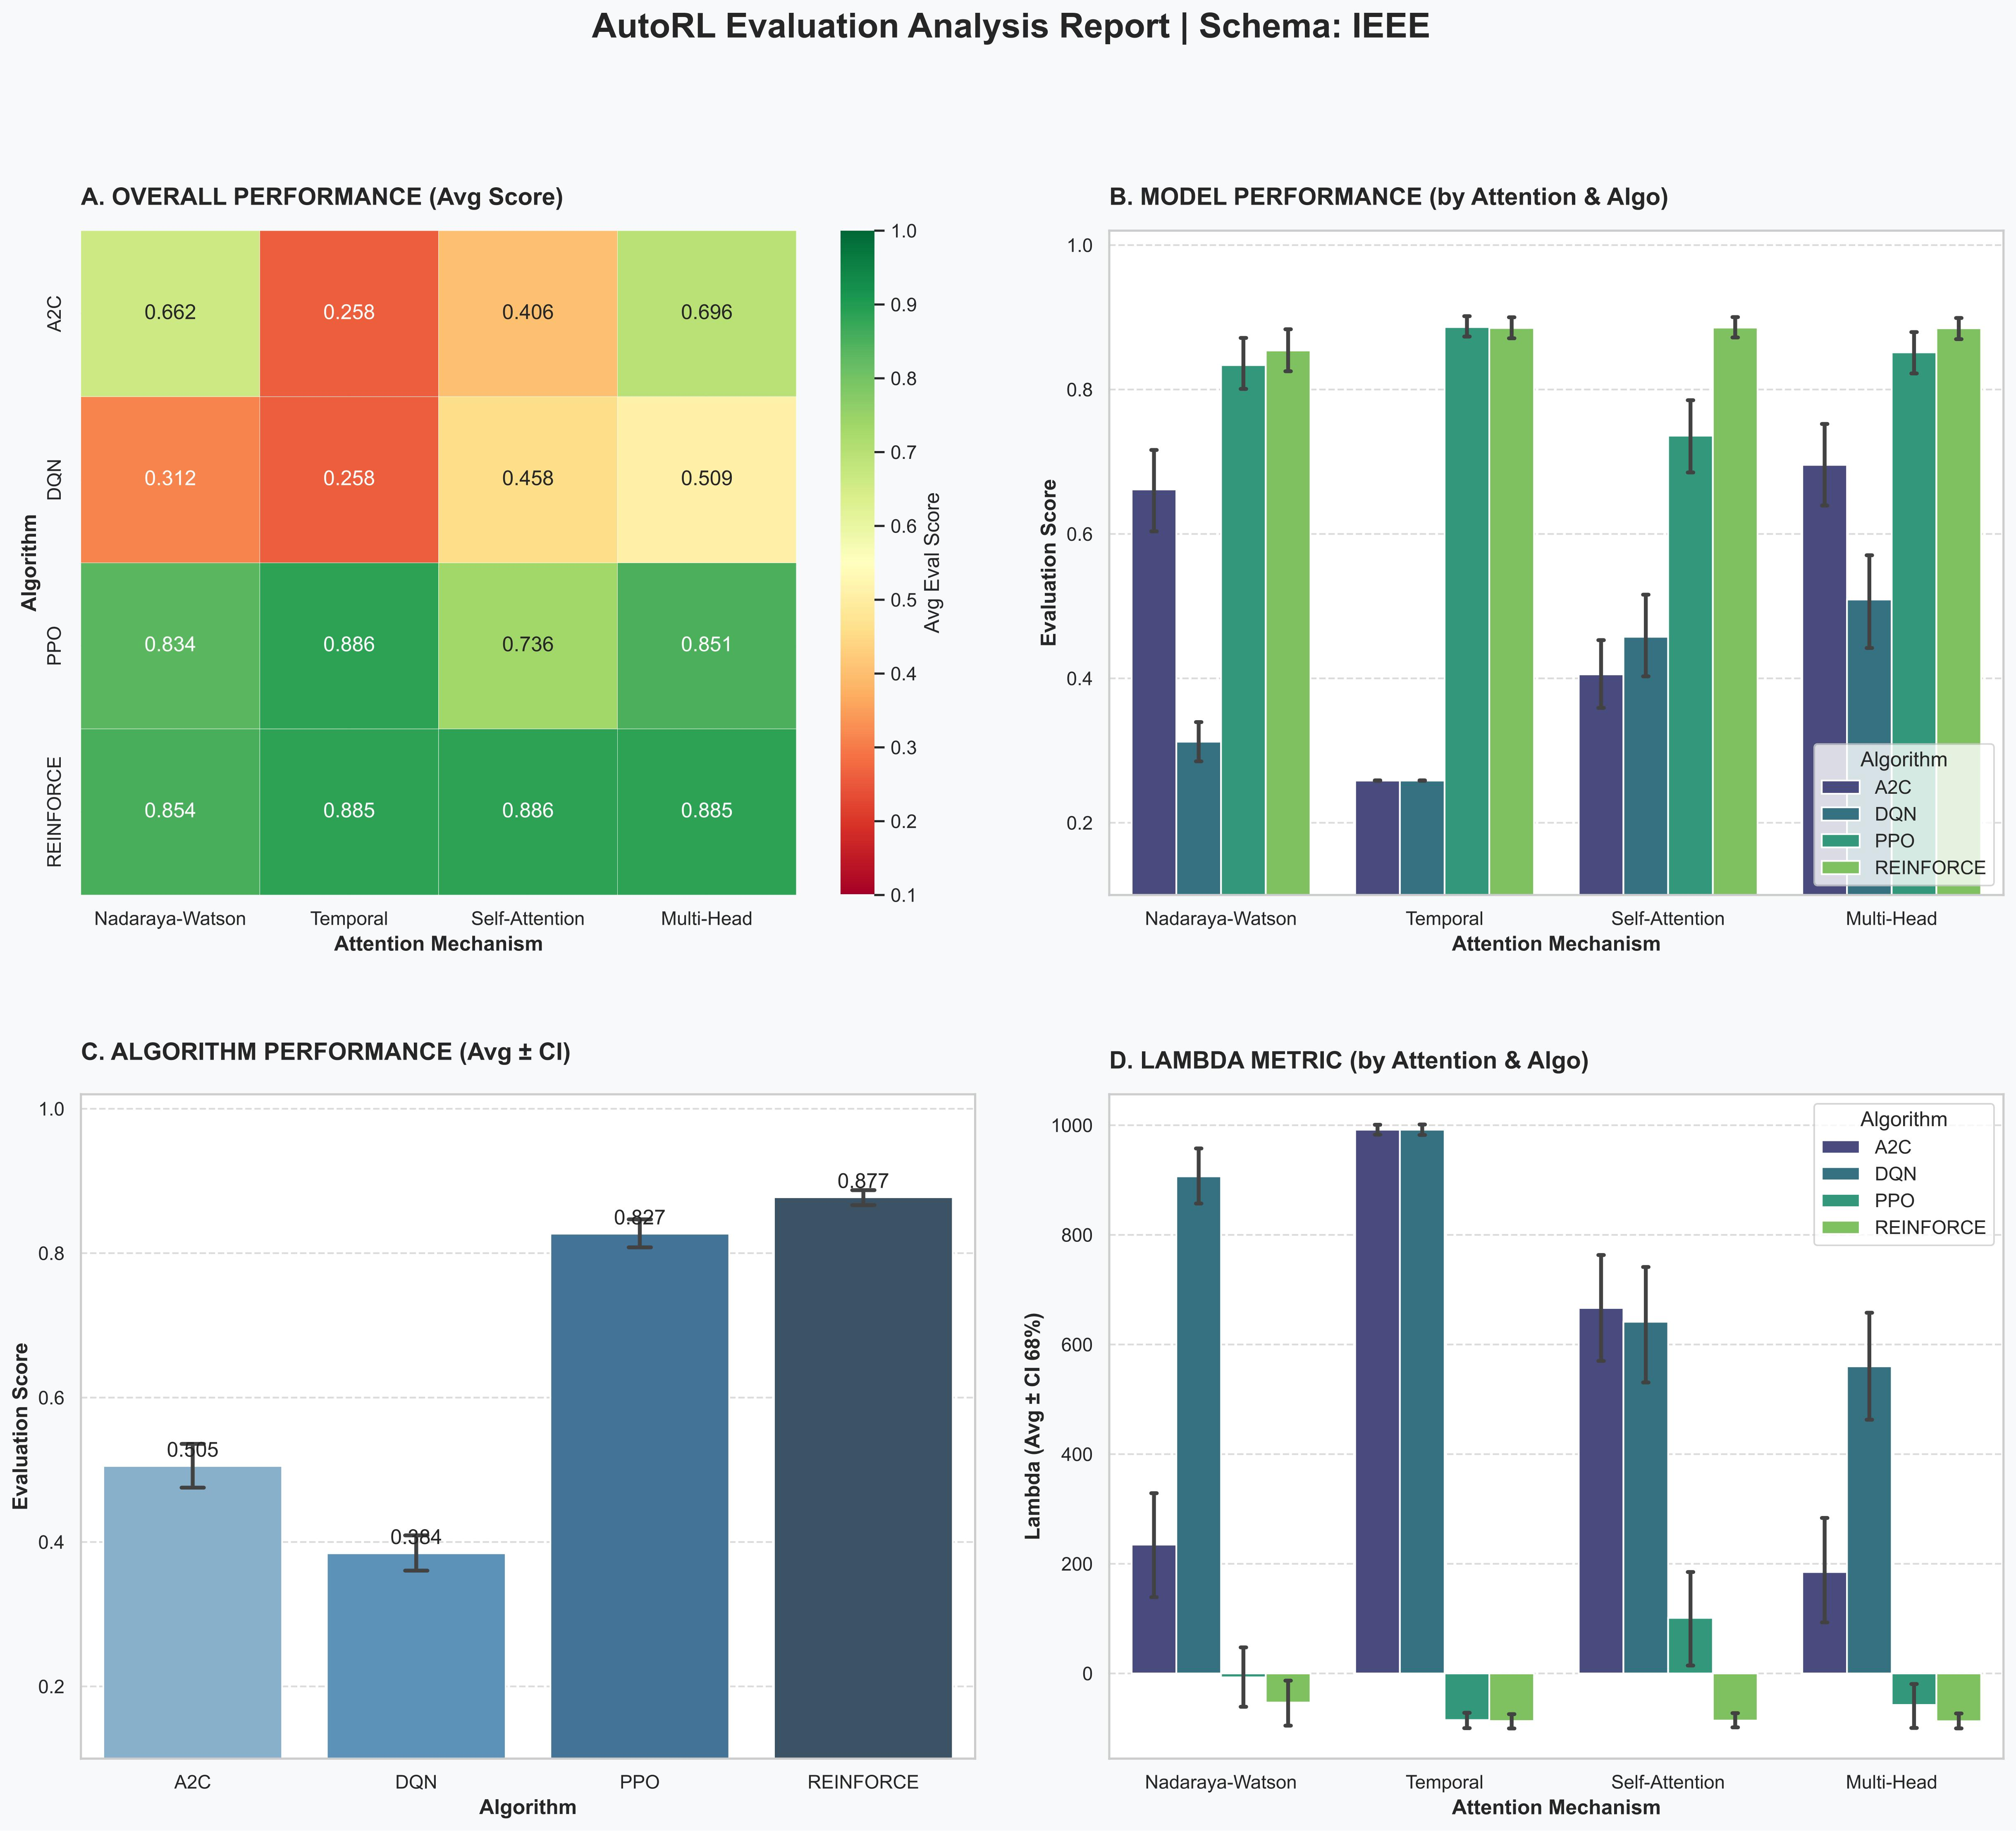
\includegraphics[width=0.95\textwidth]{_Analysis_Report_IEEE.jpg}
        \caption{Consolidated evaluation dashboard for IEEE (mean and uncertainty/error bars) used as primary visual evidence for performance patterns across algorithms and attention mechanisms.}
        \label{fig:analysis_ieee}
\end{figure}

\begin{figure}[t]
        \centering
        \includegraphics[width=0.95\textwidth,height=0.80\textheight,keepaspectratio]{_Heatmap_SIT.png}
        \caption{SIT one-vs-all generalization heatmap: trained models (rows) evaluated on unseen test files (columns).}
        \label{fig:heatmap_sit}
\end{figure}

\begin{figure}[t]
        \centering
        
\includegraphics[width=0.95\textwidth,height=0.80\textheight,keepaspectratio]{_Heatmap_IEEE.jpg}
        \caption{IEEE one-vs-all generalization heatmap: trained models (rows) evaluated on unseen test files (columns).}
        \label{fig:heatmap_ieee}
\end{figure}

%% IEEE REINFORCE + Attention
\begin{figure}[H]
  \centering
  \begin{subfigure}[t]{\textwidth}
    \centering
    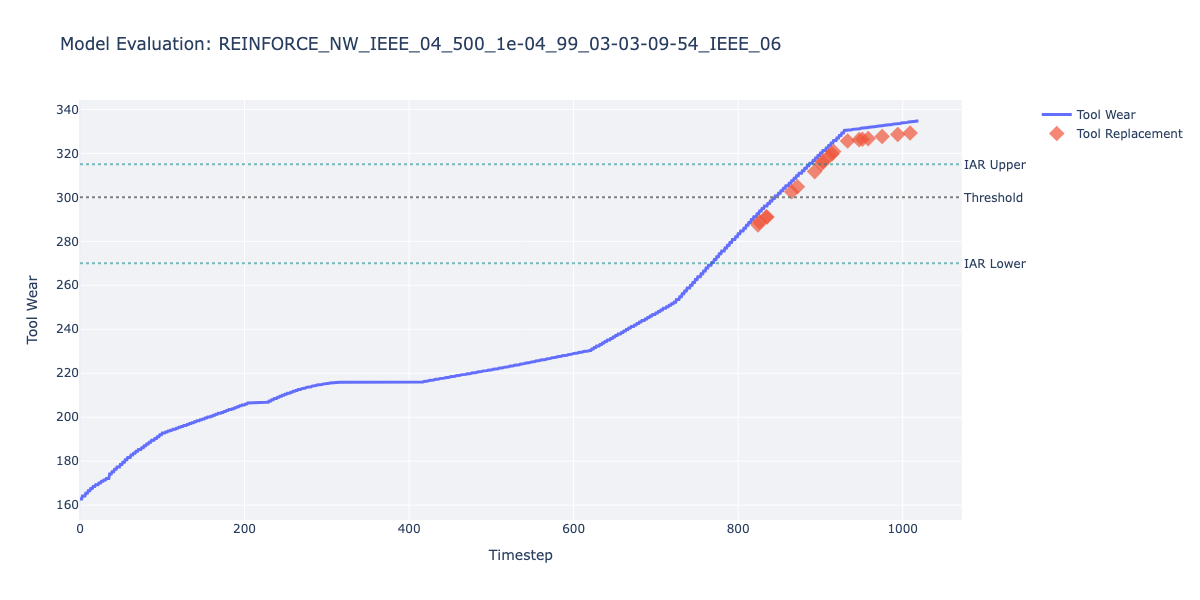
\includegraphics[width=0.8\linewidth]{REINFORCE_NW_IEEE_04_06.png}
    \caption{REINFORCE with Nadaraya--Watson attention}
    \label{fig:IEEE_RF_NW}
  \end{subfigure}
  \begin{subfigure}[t]{\textwidth}
    \centering
    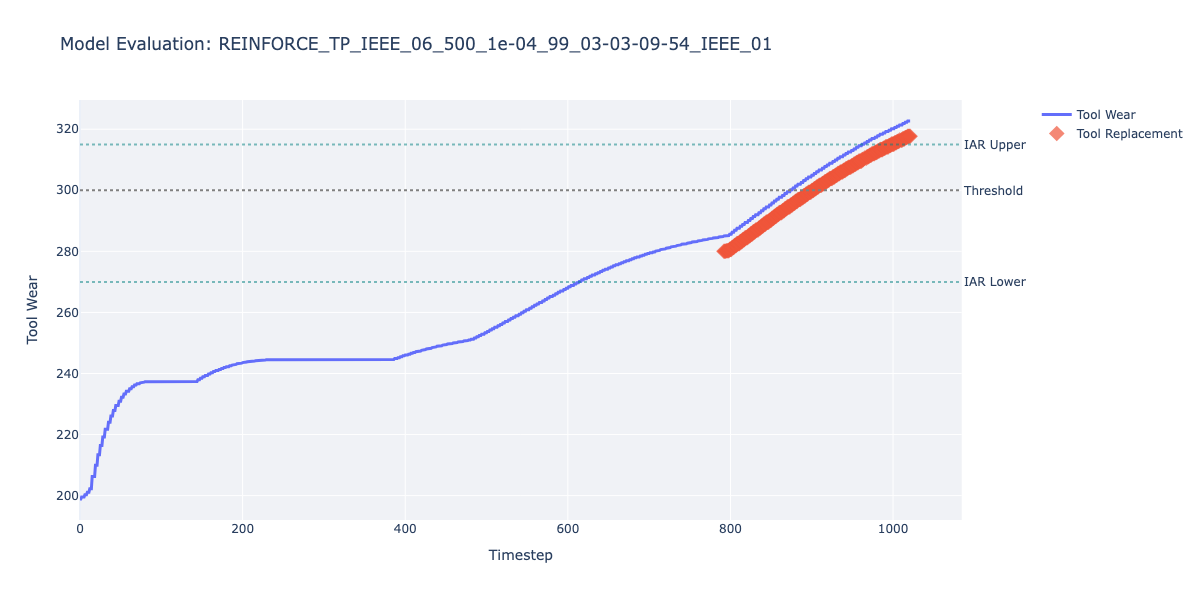
\includegraphics[width=0.8\linewidth]{REINFORCE_TP_IEEE_06_01.png}
    \caption{REINFORCE with Temporal attention}
    \label{fig:IEEE_RF_TP}
  \end{subfigure}\hfill
  \begin{subfigure}[t]{\textwidth}
    \centering
    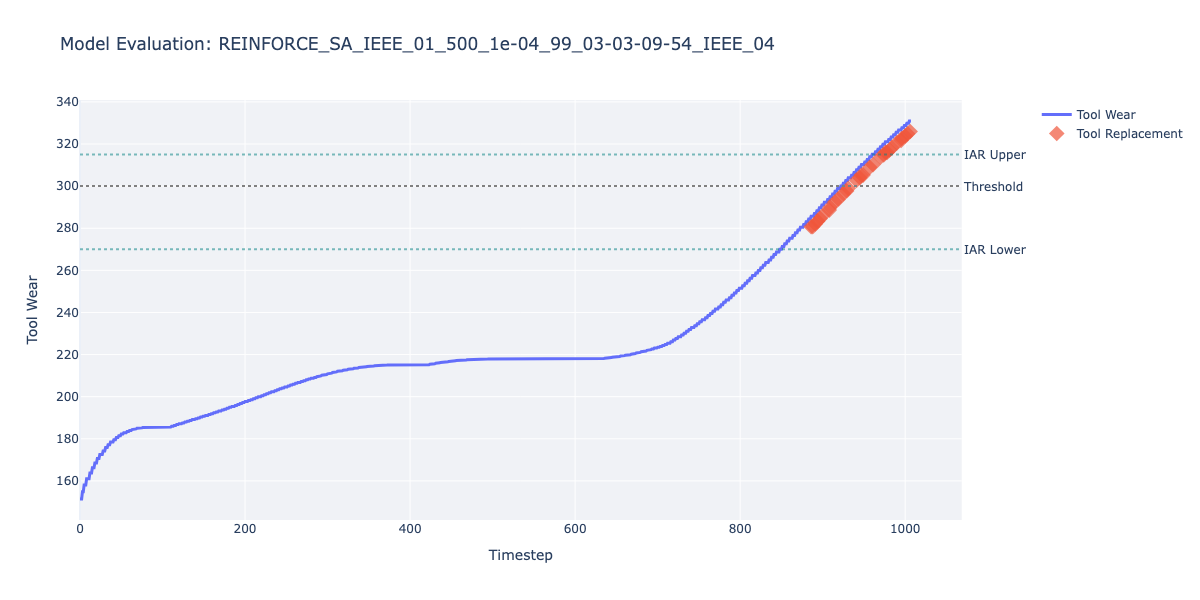
\includegraphics[width=0.8\linewidth]{REINFORCE_SA_IEEE_01_04.png}
    \caption{REINFORCE with Self-Attention}
    \label{fig:IEEE_RF_SA}
  \end{subfigure}\hfill
  \begin{subfigure}[t]{\textwidth}
    \centering
    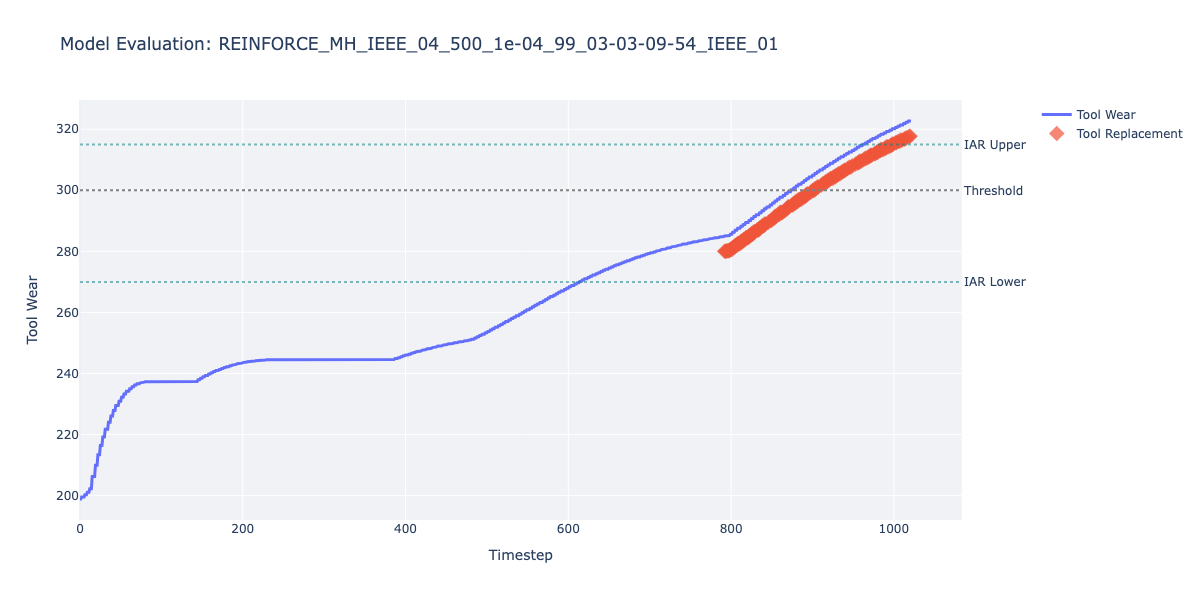
\includegraphics[width=0.8\linewidth]{REINFORCE_MH_IEEE_04_01.png}
    \caption{REINFORCE with Multi-Head attention}
    \label{fig:IEEE_RF_MH}
  \end{subfigure}

  \caption{Sample evaluation plots showing REINFORCE with different attention mechanisms, on the IEEE dataset.}
  \label{fig:IEEE_RF_with_Attention}
\end{figure}

 %% SIT REINFORCE + Attention
\begin{figure}[H]
  \centering
  \begin{subfigure}[t]{\textwidth}
    \centering
    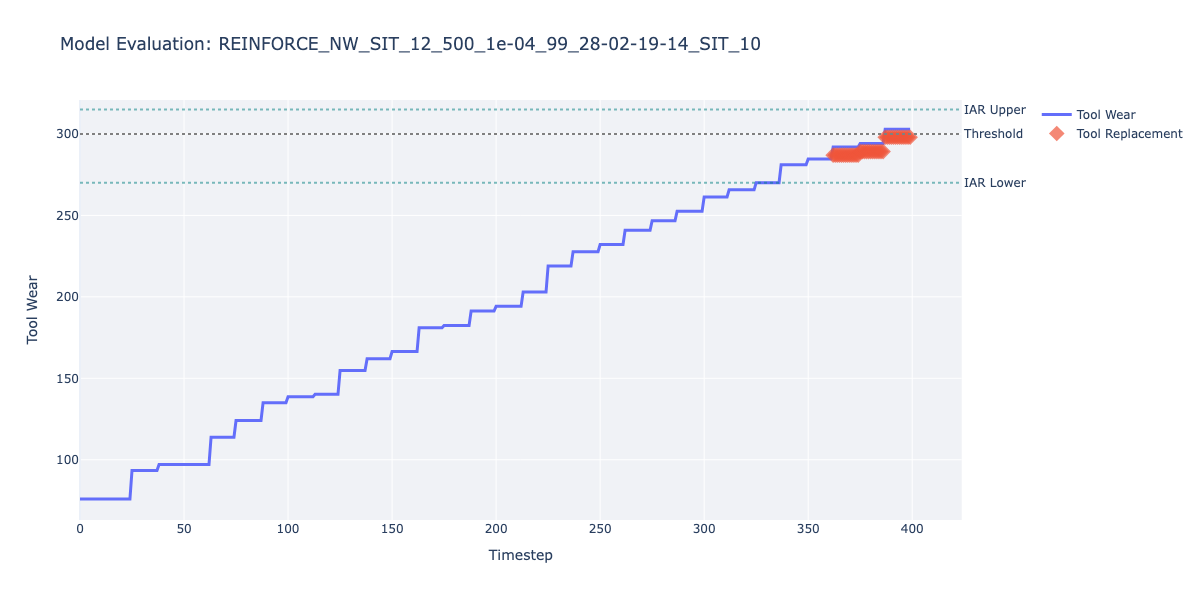
\includegraphics[width=0.8\linewidth]{REINFORCE_NW_SIT_12_10.png}
    \caption{REINFORCE with Nadaraya--Watson attention}
    \label{fig:SIT_RF_NW}
  \end{subfigure}
  \begin{subfigure}[t]{\textwidth}
    \centering
    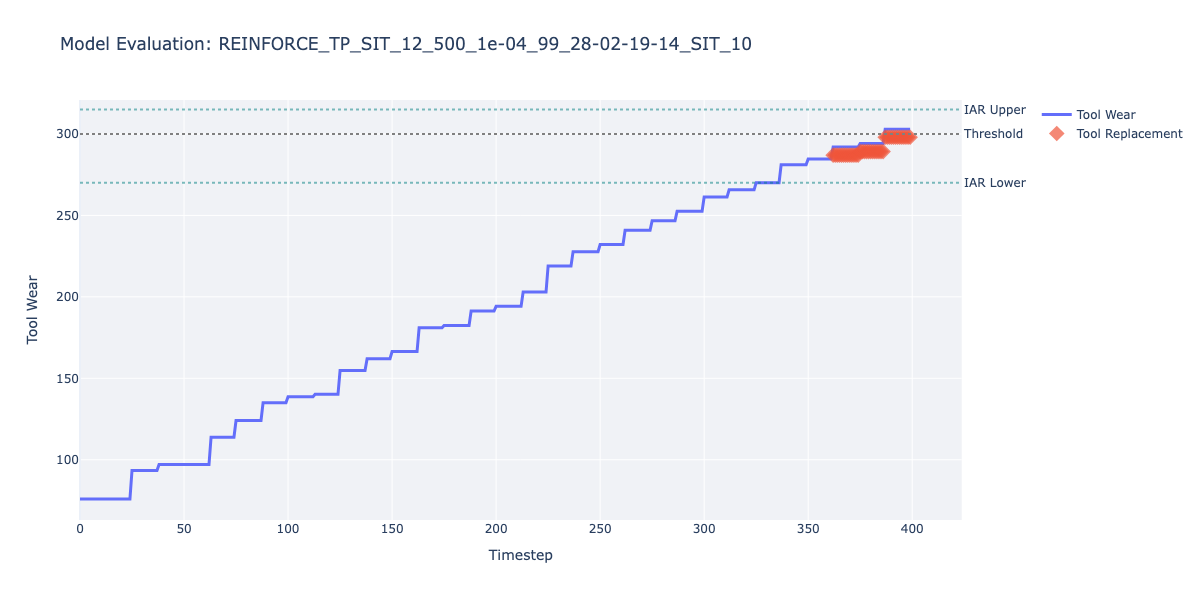
\includegraphics[width=0.8\linewidth]{REINFORCE_TP_SIT_12_10.png}
    \caption{REINFORCE with Temporal attention}
    \label{fig:SIT_RF_TP}
  \end{subfigure}\hfill
  \begin{subfigure}[t]{\textwidth}
    \centering
    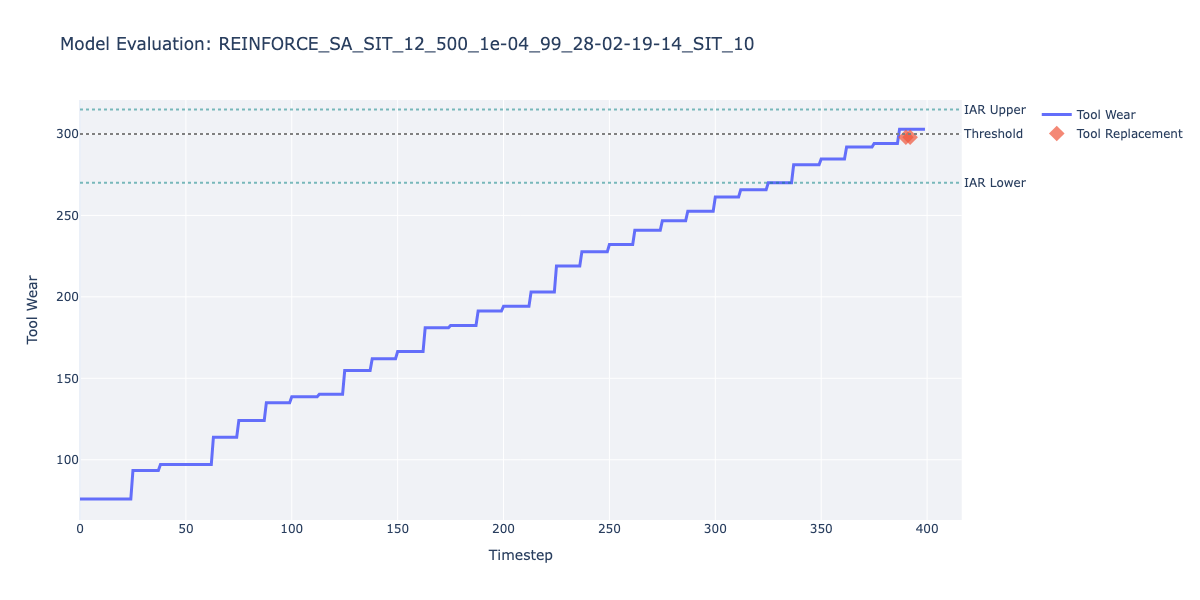
\includegraphics[width=0.8\linewidth]{REINFORCE_SA_SIT_12_10.png}
    \caption{REINFORCE with Self-Attention}
    \label{fig:SIT_RF_SA}
  \end{subfigure}
  \begin{subfigure}[t]{\textwidth}
    \centering
    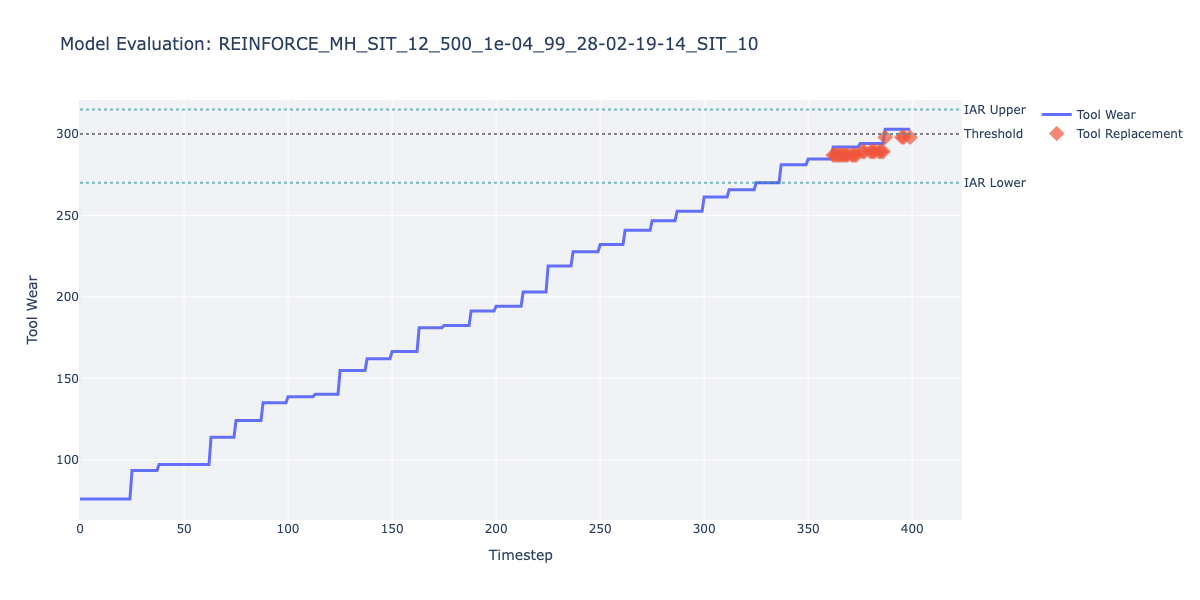
\includegraphics[width=0.8\linewidth]{REINFORCE_MH_SIT_12_10.png}
    \caption{REINFORCE with Multi-Head attention}
    \label{fig:SIT_RF_MH}
  \end{subfigure}

  \caption{Sample evaluation plots showing REINFORCE with different attention mechanisms, on the SIT dataset.}
  \label{fig:SIT_RF_with_Attention}
\end{figure}

\subsection{Hypothesis tests (H1): REINFORCE vs A2C/DQN/PPO}
\label{sec:hypothesis_tests}
The hypothesis-test artefacts provide one-tailed Welch $t$-tests at $\alpha=0.05$ for each schema. Table~\ref{tab:hyp_tests} summarizes the unseen-only evaluation-score tests for two reporting panels: \emph{All Attn} and \emph{Best Attn}.

\begin{table}[t]
        \centering
        \caption{Hypothesis tests for H1 (unseen-only evaluation score): one-tailed Welch $t$-tests comparing REINFORCE to each competitor at $\alpha=0.05$.}
        \label{tab:hyp_tests}
        % (Inlined from figures/hypothesis_tests_summary.tex)
        \begin{tabular}{l l l r r l}
        \toprule
        \textbf{Dataset} & \textbf{Panel} & \textbf{Competitor} & \textbf{t} & \textbf{p (1-tail)} & \textbf{Sig.}\\
        \midrule
        SIT & All Attn & A2C & 198.007 & 0.000 & YES\\
        SIT & Best Attn & A2C & 512.423 & 0.000 & YES\\
        SIT & All Attn & DQN & 202.449 & 0.000 & YES\\
        SIT & Best Attn & DQN & 562.313 & 0.000 & YES\\
        SIT & All Attn & PPO & 20.686 & 0.000 & YES\\
        SIT & Best Attn & PPO & 49.902 & 0.000 & YES\\
        IEEE & All Attn & A2C & 10.726 & 0.000 & YES\\
        IEEE & Best Attn & A2C & 10.434 & 0.000 & YES\\
        IEEE & All Attn & DQN & 15.977 & 0.000 & YES\\
        IEEE & Best Attn & DQN & 15.235 & 0.000 & YES\\
        IEEE & All Attn & PPO & 1.957 & 0.026 & YES\\
        IEEE & Best Attn & PPO & 2.096 & 0.020 & YES\\
        \bottomrule
        \end{tabular}
\end{table}

\subsection{Quantitative IEEE summary (means and 95\% CI)}
\label{sec:ieee_summary}
Table~\ref{tab:ieee_top10} lists the top IEEE configurations by mean evaluation score, and Table~\ref{tab:ieee_best_attn} summarizes the best attention mechanism per algorithm.

\begin{table}[t]
        \centering
        \caption{Top IEEE configurations on unseen-only evaluations (mean and 95\% CI, aggregated across trained models and test files). Numbers are rounded to three decimals.}
        \label{tab:ieee_top10}
        % (Inlined from figures/ieee_unseen_summary.tex)
        \begin{tabular}{ll r r r r}
        \toprule
        \textbf{Algorithm} & \textbf{Attention} & \textbf{Eval. Score} & \textbf{CI} & \textbf{Tool use (\%)} & \textbf{$\lambda$}\\
        \midrule
        PPO & Temporal & 0.886 & 0.031 & 95.199 & -85.050\\
        REINFORCE & Multi-Head & 0.886 & 0.031 & 95.215 & -85.700\\
        REINFORCE & Self-Attention & 0.886 & 0.031 & 95.261 & -86.100\\
        REINFORCE & Temporal & 0.885 & 0.031 & 95.341 & -86.750\\
        PPO & Nadaraya-Watson & 0.857 & 0.070 & 93.651 & -31.900\\
        REINFORCE & Nadaraya-Watson & 0.850 & 0.068 & 93.079 & -40.950\\
        PPO & Multi-Head & 0.843 & 0.070 & 93.170 & -50.300\\
        PPO & Self-Attention & 0.740 & 0.114 & 87.271 & 109.150\\
        A2C & Multi-Head & 0.684 & 0.130 & 82.617 & 208.600\\
        A2C & Nadaraya-Watson & 0.669 & 0.129 & 83.096 & 212.750\\
        \bottomrule
        \end{tabular}
\end{table}

\begin{table}[t]
        \centering
        \caption{IEEE unseen-only: best attention mechanism per algorithm (mean evaluation score and 95\% CI).}
        \label{tab:ieee_best_attn}
        % (Inlined from figures/ieee_best_attention_per_algo.tex)
        \begin{tabular}{l l r r r}
        \toprule
        \textbf{Algorithm} & \textbf{Best attention} & \textbf{Eval. Score} & \textbf{CI} & \textbf{n}\\
        \midrule
        A2C & Multi-Head & 0.684 & 0.130 & 20\\
        DQN & Multi-Head & 0.509 & 0.139 & 20\\
        PPO & Temporal & 0.886 & 0.031 & 20\\
        REINFORCE & Multi-Head & 0.886 & 0.031 & 20\\
        \bottomrule
        \end{tabular}
\end{table}

\subsection{Statistical heatmaps: p-values and t-statistics}
\textbf{Dataset-level interpretation.}
\textbf{SIT (consolidated).} The SIT dashboard (Figure~\ref{fig:analysis_sit}) indicates a clear separation between the two lightweight baselines (A2C/DQN) and the two top performers (PPO/\textsc{REINFORCE}) across attention mechanisms.

\textbf{IEEE.} IEEE results show a tighter competition between PPO and \textsc{REINFORCE}, with the best-attention panel identifying self-attention as a strong \textsc{REINFORCE} configuration (Tables~\ref{tab:ieee_top10}--\ref{tab:ieee_best_attn}).

\textbf{Attention improves REINFORCE (H3).}
Across schemas, multi-head attention emerges as the best or most consistent attention mechanism in the statistical panels and the consolidated analysis reports.

\textbf{Practical recommendation.}
For edge-first deployments where training and inference budgets are constrained, the evidence supports a simple default: \emph{REINFORCE + Multi-Head attention}. When a practitioner has bandwidth to benchmark alternatives, PPO with temporal attention is a strong secondary candidate.

\subsection{H2: cross-schema generality (SIT vs IEEE)}
H2 is supported structurally by the environment design (Section~\ref{sec:env}) and empirically by results on both schemas (Figures~\ref{fig:analysis_sit}--\ref{fig:heatmap_ieee}). The same environment class (with schema detection and feature selection) and the same reward shaping (Section~\ref{sec:reward}) produce strong-performing agents in both SIT and IEEE settings.
\begin{figure}[t]
        \centering
        \includegraphics[width=0.95\textwidth]{_Statistical_p-value_SIT.png}
        \caption{SIT $p$-value heatmap for hypothesis tests (blue indicates stronger evidence).}
        \label{fig:pvalues_sit}
\end{figure}

\begin{figure}[t]
        \centering
        \includegraphics[width=0.95\textwidth]{_Statistical_p-value_IEEE.jpg}
        \caption{IEEE $p$-value heatmap for hypothesis tests (blue indicates stronger evidence).}
        \label{fig:pvalues_ieee}
\end{figure}

\begin{figure}[t]
        \centering
        \includegraphics[width=0.95\textwidth]{_Statistical_t_SIT.png}
        \caption{SIT $t$-statistic heatmap corresponding to Figure~\ref{fig:pvalues_sit}.}
        \label{fig:tstats_sit}
\end{figure}

\begin{figure}[t]
        \centering
        \includegraphics[width=0.95\textwidth]{_Statistical_t_IEEE.jpg}
        \caption{IEEE $t$-statistic heatmap corresponding to Figure~\ref{fig:pvalues_ieee}.}
        \label{fig:tstats_ieee}
\end{figure}

\section{Discussion}
\label{sec:discussion}
\subsection{Why lightweight REINFORCE can win in this PdM setup}
The PdM task studied here has a small action space and terminates on replacement; accordingly, the control problem can resemble learning a decision boundary over sensor-derived features. When partial observability dominates the difficulty (Section~\ref{sec:pomdp}), representation quality can matter more than optimizer sophistication.

\subsection{Implications for industrial practitioners}
The primary practical implication is that a lightweight policy-gradient learner (\textsc{REINFORCE}), when paired with appropriate attention-based feature extraction, can be a credible choice for edge-first PdM deployments where model footprint and operational simplicity matter. AutoRL is therefore framed as a \emph{convenience layer}: it reduces reliance on RL expertise by automating algorithm/attention sweeps and exposing standardized result artefacts (dashboards, heatmaps, and hypothesis-test summaries) for selection and auditing.

\subsection{Edge compute and sustainability framing}
This paper does not directly measure energy consumption. However, the combination of AutoRL-style sweeps and edge deployment makes compute-efficiency a meaningful engineering constraint. In this context, if REINFORCE achieves equal or better PdM outcomes than heavier baselines, it supports a defensible ``Green AI'' argument: prefer the simplest method that meets the operational objective \cite{Schwartz2020, Strubell2019}.

\section{Limitations and threats to validity}
\label{sec:limits}
\begin{itemize}
        \item \textbf{Dataset-driven environment:} the environment replays logged runs-to-threshold and does not model intervention dynamics beyond termination; future work can extend to maintenance logistics and downtime costs.
        \item \textbf{Temporal extractor state:} temporal attention maintains an internal timestep counter; production use should ensure the counter resets consistently with episode resets.
        \item \textbf{Compute and carbon measurement:} energy/carbon implications are argued from algorithmic complexity and deployment constraints rather than measured on edge hardware.
\end{itemize}

\section{Conclusions and future work}
\label{sec:conclusion}
This paper presented an empirical study of \textsc{REINFORCE} with attention mechanisms for milling-machine tool-replacement PdM under edge-oriented constraints, using a schema-adaptive Gymnasium environment and multi-round evaluation on unseen data. Results across SIT and IEEE schemas, supported by hypothesis tests at $\alpha=0.05$, show that \textsc{REINFORCE} is a strong candidate for edge-first PdM, and that attention mechanisms---especially multi-head attention---can further improve performance and robustness. AutoRL is used as an implementation mechanism to standardize sweeps and reporting rather than as the core research contribution.

Future work should (i) measure inference latency and energy on representative edge devices, (ii) incorporate richer maintenance costs and partial observability models, and (iii) evaluate robustness under sensor drift and cross-machine domain shift.



\section*{Acknowledgements}

Acknowledgements are not compulsory. Where included they should be brief. Grant or contribution numbers may be acknowledged.

Please refer to Journal-level guidance for any specific requirements.

\section*{Declarations}

\subsection*{Funding}

\subsection*{Conflict of interest/Competing interests}
Not applicable

\subsection*{Ethics approval and consent to participate}
Not applicable

\subsection*{Consent for publication}
xxxx

\subsection*{Data availability}
xxxx

\subsection*{Materials availability}
Not applicable

\subsection*{Code availability}

\subsection*{Author contribution}
\begin{itemize}
        \item Conceptualization: Rajesh Siraskar, Satish Kumar
        \item Methodology: Rajesh Siraskar, Satish Kumar, Shruti Patil
\end{itemize}

\begin{appendices}

\section{Environment and reward details}
\label{app:env_reward}
\subsection{Observation design and POMDP rationale}
The environment returns observation vectors comprised only of sensor channels. Tool wear is excluded from observations but is used internally to compute termination and reward.

\subsection{Reward components}
\begin{table}[t]
        \centering
        \caption{Reward shaping components in the milling PdM environment (qualitative summary).}
        \label{tab:reward_components}
        \begin{tabular}{p{0.20\linewidth} p{0.22\linewidth} p{0.50\linewidth}}
                \toprule
                \textbf{Component} & \textbf{Applied when} & \textbf{Effect}\\
                \midrule
                $R_1$ survival reward & continue and safe & Encourages utilization while below threshold.\\
                $R_2$ violation penalty & continue and violate & Strongly discourages threshold violation.\\
                $R_3$ replacement cost & replace action & Regularizes against replacing too early.\\
                $R_4$ near-threshold bonus & replace near $\tau$ & Rewards timely replacement close to threshold.\\
                Stepwise bonuses & wear ratio $\,\ge 0.7, 0.8, 0.9$ & Increases incentive as wear approaches threshold.\\
                \bottomrule
        \end{tabular}
\end{table}

\section{Evaluation protocol details}
\label{app:eval}
\subsection{Multi-round evaluation}
Each agent is evaluated for multiple rounds per test file to reduce variance due to stochastic policies and initialization.

\subsection{Unseen-only emphasis}
This paper focuses on unseen-only evaluation panels for generalization claims (H2). Panels that include self-evaluation are useful for debugging and sanity checks but can overestimate deployment performance.

\section{Dataset schemas and sensor signals}
\label{app:schema}
\begin{table}[t]
\centering
\caption{Sensor channels used as observations by schema (as implemented in \texttt{MT\_Env}).}
\label{tab:schema_features}
\begin{tabular}{p{0.18\linewidth} p{0.75\linewidth}}
\toprule
\textbf{Schema} & \textbf{Observation channels}\\
\midrule
SIT & \texttt{Vib\_Spindle}, \texttt{Vib\_Table}, \texttt{Sound\_Spindle}, \texttt{Sound\_table}, \texttt{X\_Load\_Cell}, \texttt{Y\_Load\_Cell}, \texttt{Z\_Load\_Cell}, \texttt{Current}\\
IEEE & \texttt{force\_x}, \texttt{force\_y}, \texttt{force\_z}, \texttt{vibration\_x}, \texttt{vibration\_y}, \texttt{vibration\_z}, \texttt{acoustic\_emission\_rms}\\
\bottomrule
\end{tabular}
\end{table}

\section{Default constants and hyperparameters}
\label{app:defaults}
\begin{table}[t]
\centering
\caption{Default environment/training constants (from \texttt{code/rl\_pdm.py} and \texttt{code/batch\_train.py}).}
\label{tab:defaults}
\begin{tabular}{p{0.34\linewidth} p{0.18\linewidth} p{0.40\linewidth}}
\toprule
\textbf{Parameter} & \textbf{Default} & \textbf{Meaning}\\
\midrule
\texttt{WEAR\_THRESHOLD} & 300.000 & Wear threshold used for termination and reporting.\\
\texttt{TRAINING\_WEAR\_THRESHOLD} & 300.000 & Training threshold (configurable; default equals threshold).\\
\texttt{EPISODES} & 100 & Training episodes per run (default in RL module).\\
\texttt{LR\_DEFAULT} & 0.001 & Default learning rate (overridden by AutoRL sweep values).\\
\texttt{GAMMA\_DEFAULT} & 0.990 & Default discount factor (overridden by AutoRL sweep values).\\
\texttt{EVAL\_ROUNDS} & 20 & Evaluation rounds per model on unseen data.\\
\texttt{IAR\_RANGE} & 0.050 & IAR bounds range for timing metric computation.\\
\texttt{LAMBDA} & 0.900 & Logistic slack coefficient used in $\lambda$ timing computation.\\
\texttt{R1}, \texttt{R2}, \texttt{R3}, \texttt{R4} & 0.100, -100.000, -0.500, 60.000 & Reward shaping constants.\\
\bottomrule
\end{tabular}
\end{table}

\section{Core code implementation snippets}
\label{app:code_snippets}

\subsection{Nadaraya--Watson attention: forward pass}
\begin{lstlisting}[language=Python,caption={NadarayaWatsonExtractor.forward (code/rl\_pdm.py)},label={lst:nw_forward}]
# NadarayaWatsonExtractor.forward (code/rl_pdm.py)
query = self.query_net(observations)          # q
dist  = (query.unsqueeze(1) - self.keys.unsqueeze(0)).pow(2).sum(dim=2)
beta  = th.exp(self.log_beta)                 # beta > 0
alpha = th.softmax(-beta * dist, dim=1)       # softmax over prototypes
context = (alpha.unsqueeze(2) * self.values.unsqueeze(0)).sum(dim=1)
return context
\end{lstlisting}

\subsection{Temporal attention: forward pass}
\begin{lstlisting}[language=Python,caption={TemporalAttentionExtractor.forward (code/rl\_pdm.py)},label={lst:tp_forward}]
# TemporalAttentionExtractor.forward (code/rl_pdm.py)
spatial_weights = self.spatial_attention(observations)
weighted_spatial = observations * spatial_weights

timestep_idx = int(self.current_timestep.item()) % self.max_timesteps
temporal_encoding = self.positional_encoding[timestep_idx]
temporal_features = temporal_encoding + self.temporal_embedding

combined = th.cat([weighted_spatial, temporal_features.expand(batch_size, -1)], dim=1)
output = self.fusion_net(combined)
self.current_timestep += 1
return output
\end{lstlisting}

\subsection{Multi-head attention: forward pass}
\begin{lstlisting}[language=Python,caption={MultiHeadAttentionExtractor.forward (code/rl\_pdm.py)},label={lst:mh_forward}]
# MultiHeadAttentionExtractor.forward (code/rl_pdm.py)
Q = self.query_proj(observations).view(batch, H, d)
K = self.key_proj(observations).view(batch, H, d)
V = self.value_proj(observations).view(batch, H, d)

scores  = th.einsum('bhd,bhd->bh', Q, K) * self.scale
alpha_h = th.softmax(scores, dim=1).unsqueeze(2)    # softmax over heads
attended = alpha_h * V
concat = attended.view(batch, H * d)
return self.output_proj(concat)
\end{lstlisting}

\subsection{Self-attention: forward pass}
\begin{lstlisting}[language=Python,caption={SelfAttentionExtractor.forward (code/rl\_pdm.py)},label={lst:sa_forward}]
# SelfAttentionExtractor.forward (code/rl_pdm.py)
x = self.input_proj(observations)
Q = self.query(x); K = self.key(x); V = self.value(x)

scores = (Q * K).sum(dim=1, keepdim=True) * self.scale
alpha  = th.softmax(scores, dim=0)          # normalize across batch
attn_output = alpha * V

x = self.norm1(x + attn_output)
x = self.norm2(x + self.ffn(x))
return x
\end{lstlisting}

\subsection{Evaluation score: reference implementation}
\begin{lstlisting}[language=Python,caption={calculate\_eval\_score (code/batch\_train.py)},label={lst:eval_score}]
# calculate_eval_score (code/batch_train.py)
tool_usage_score = min(1.0, max(0.0, tool_usage_pct))
IAR_LOWER = rl_pdm.WEAR_THRESHOLD * (1.0 - rl_pdm.IAR_RANGE)
lambda_score = max(0.0, 1.0 - (abs(lambda_metric) / IAR_LOWER))
violation_score = max(0.0, 1.0 / (1.0 + violations))
eval_score = 0.50*tool_usage_score + 0.30*lambda_score + 0.20*violation_score
\end{lstlisting}

\end{appendices}

\bibliography{JoIM_references}

\end{document}
